% Options for packages loaded elsewhere
\PassOptionsToPackage{unicode}{hyperref}
\PassOptionsToPackage{hyphens}{url}
\PassOptionsToPackage{dvipsnames,svgnames,x11names}{xcolor}
\documentclass[
  10pt,
]{article}
\usepackage{xcolor}
\usepackage[margin=1in]{geometry}
\usepackage{amsmath,amssymb}
\setcounter{secnumdepth}{-\maxdimen} % remove section numbering
\usepackage{iftex}
\ifPDFTeX
  \usepackage[T1]{fontenc}
  \usepackage[utf8]{inputenc}
  \usepackage{textcomp} % provide euro and other symbols
\else % if luatex or xetex
  \usepackage{unicode-math} % this also loads fontspec
  \defaultfontfeatures{Scale=MatchLowercase}
  \defaultfontfeatures[\rmfamily]{Ligatures=TeX,Scale=1}
\fi
\usepackage{lmodern}
\ifPDFTeX\else
  % xetex/luatex font selection
\fi
% Use upquote if available, for straight quotes in verbatim environments
\IfFileExists{upquote.sty}{\usepackage{upquote}}{}
\IfFileExists{microtype.sty}{% use microtype if available
  \usepackage[]{microtype}
  \UseMicrotypeSet[protrusion]{basicmath} % disable protrusion for tt fonts
}{}
\makeatletter
\@ifundefined{KOMAClassName}{% if non-KOMA class
  \IfFileExists{parskip.sty}{%
    \usepackage{parskip}
  }{% else
    \setlength{\parindent}{0pt}
    \setlength{\parskip}{6pt plus 2pt minus 1pt}}
}{% if KOMA class
  \KOMAoptions{parskip=half}}
\makeatother
\usepackage{color}
\usepackage{fancyvrb}
\newcommand{\VerbBar}{|}
\newcommand{\VERB}{\Verb[commandchars=\\\{\}]}
\DefineVerbatimEnvironment{Highlighting}{Verbatim}{commandchars=\\\{\}}
% Add ',fontsize=\small' for more characters per line
\newenvironment{Shaded}{}{}
\newcommand{\AlertTok}[1]{\textcolor[rgb]{1.00,0.00,0.00}{\textbf{#1}}}
\newcommand{\AnnotationTok}[1]{\textcolor[rgb]{0.38,0.63,0.69}{\textbf{\textit{#1}}}}
\newcommand{\AttributeTok}[1]{\textcolor[rgb]{0.49,0.56,0.16}{#1}}
\newcommand{\BaseNTok}[1]{\textcolor[rgb]{0.25,0.63,0.44}{#1}}
\newcommand{\BuiltInTok}[1]{\textcolor[rgb]{0.00,0.50,0.00}{#1}}
\newcommand{\CharTok}[1]{\textcolor[rgb]{0.25,0.44,0.63}{#1}}
\newcommand{\CommentTok}[1]{\textcolor[rgb]{0.38,0.63,0.69}{\textit{#1}}}
\newcommand{\CommentVarTok}[1]{\textcolor[rgb]{0.38,0.63,0.69}{\textbf{\textit{#1}}}}
\newcommand{\ConstantTok}[1]{\textcolor[rgb]{0.53,0.00,0.00}{#1}}
\newcommand{\ControlFlowTok}[1]{\textcolor[rgb]{0.00,0.44,0.13}{\textbf{#1}}}
\newcommand{\DataTypeTok}[1]{\textcolor[rgb]{0.56,0.13,0.00}{#1}}
\newcommand{\DecValTok}[1]{\textcolor[rgb]{0.25,0.63,0.44}{#1}}
\newcommand{\DocumentationTok}[1]{\textcolor[rgb]{0.73,0.13,0.13}{\textit{#1}}}
\newcommand{\ErrorTok}[1]{\textcolor[rgb]{1.00,0.00,0.00}{\textbf{#1}}}
\newcommand{\ExtensionTok}[1]{#1}
\newcommand{\FloatTok}[1]{\textcolor[rgb]{0.25,0.63,0.44}{#1}}
\newcommand{\FunctionTok}[1]{\textcolor[rgb]{0.02,0.16,0.49}{#1}}
\newcommand{\ImportTok}[1]{\textcolor[rgb]{0.00,0.50,0.00}{\textbf{#1}}}
\newcommand{\InformationTok}[1]{\textcolor[rgb]{0.38,0.63,0.69}{\textbf{\textit{#1}}}}
\newcommand{\KeywordTok}[1]{\textcolor[rgb]{0.00,0.44,0.13}{\textbf{#1}}}
\newcommand{\NormalTok}[1]{#1}
\newcommand{\OperatorTok}[1]{\textcolor[rgb]{0.40,0.40,0.40}{#1}}
\newcommand{\OtherTok}[1]{\textcolor[rgb]{0.00,0.44,0.13}{#1}}
\newcommand{\PreprocessorTok}[1]{\textcolor[rgb]{0.74,0.48,0.00}{#1}}
\newcommand{\RegionMarkerTok}[1]{#1}
\newcommand{\SpecialCharTok}[1]{\textcolor[rgb]{0.25,0.44,0.63}{#1}}
\newcommand{\SpecialStringTok}[1]{\textcolor[rgb]{0.73,0.40,0.53}{#1}}
\newcommand{\StringTok}[1]{\textcolor[rgb]{0.25,0.44,0.63}{#1}}
\newcommand{\VariableTok}[1]{\textcolor[rgb]{0.10,0.09,0.49}{#1}}
\newcommand{\VerbatimStringTok}[1]{\textcolor[rgb]{0.25,0.44,0.63}{#1}}
\newcommand{\WarningTok}[1]{\textcolor[rgb]{0.38,0.63,0.69}{\textbf{\textit{#1}}}}
\usepackage{longtable,booktabs,array}
\newcounter{none} % for unnumbered tables
\usepackage{calc} % for calculating minipage widths
% Correct order of tables after \paragraph or \subparagraph
\usepackage{etoolbox}
\makeatletter
\patchcmd\longtable{\par}{\if@noskipsec\mbox{}\fi\par}{}{}
\makeatother
% Allow footnotes in longtable head/foot
\IfFileExists{footnotehyper.sty}{\usepackage{footnotehyper}}{\usepackage{footnote}}
\makesavenoteenv{longtable}
\usepackage{graphicx}
\makeatletter
\newsavebox\pandoc@box
\newcommand*\pandocbounded[1]{% scales image to fit in text height/width
  \sbox\pandoc@box{#1}%
  \Gscale@div\@tempa{\textheight}{\dimexpr\ht\pandoc@box+\dp\pandoc@box\relax}%
  \Gscale@div\@tempb{\linewidth}{\wd\pandoc@box}%
  \ifdim\@tempb\p@<\@tempa\p@\let\@tempa\@tempb\fi% select the smaller of both
  \ifdim\@tempa\p@<\p@\scalebox{\@tempa}{\usebox\pandoc@box}%
  \else\usebox{\pandoc@box}%
  \fi%
}
% Set default figure placement to htbp
\def\fps@figure{htbp}
\makeatother
\setlength{\emergencystretch}{3em} % prevent overfull lines
\providecommand{\tightlist}{%
  \setlength{\itemsep}{0pt}\setlength{\parskip}{0pt}}
\usepackage{fvextra}
\DefineVerbatimEnvironment{Highlighting}{Verbatim}{breaklines,breakanywhere,commandchars=\\\{\}}
\fvset{breaklines,breakanywhere}
\usepackage{bookmark}
\IfFileExists{xurl.sty}{\usepackage{xurl}}{} % add URL line breaks if available
\urlstyle{same}
\hypersetup{
  colorlinks=true,
  linkcolor={Maroon},
  filecolor={Maroon},
  citecolor={Blue},
  urlcolor={Blue},
  pdfcreator={LaTeX via pandoc}}

\author{}
\date{}

\begin{document}

\section{Lemma: Verified LLM Synthesis of Query
Executors}\label{lemma-verified-llm-synthesis-of-query-executors}

Oct 11, 2026 \ensuremath{\cdot} @Emil

Draft for VLDB (PVLDB template), moved here from
LEMMA\_PAPER\_111026.tex to write and add figures; LaTeX comes back at
the end.

\subsection{Abstract}\label{abstract}

General-purpose OLAP engines pay for their generality through
interpretation, generic operators, and layers of abstraction. Recent
systems show that LLM-synthesized, per-query executors can be far
faster, but their correctness rests on tests and inspection, so a single
wrong answer can go unnoticed. We present Lemma, a query engine that
pairs LLM synthesis with machine-checked proof. Lemma deterministically
transpiles each SQL query and its catalog schema into a formal
specification in Verus, a verifier for Rust. An LLM agent then writes an
optimized native executor for that query and uses Verus to prove the
executor equivalent to the specification before it is compiled and
served. An executor can only run once it's been verified. Verified
binaries are cached and invoked from a DuckDB extension, so recurring
analytical queries amortize the one-time cost of synthesis and proof. On
TPC-H and the Star Schema Benchmark, Lemma proves {[}TBA{]}\% of the
queries it accepts, and its verified executors run {[}TBA{]}\ensuremath{\times} faster
than all-core DuckDB on hot runs. To our knowledge, Lemma is the first
query engine whose LLM-written executors are formally proved equivalent
to the query's specification.

\subsection{Introduction}\label{introduction}

\begin{itemize}
\tightlist
\item
  General-purpose OLAP engines pay for generality (interpretation,
  operators, abstractions).
\item
  LLM-synthesized per-query code can be much faster (CodexDB, GenDB,
  Bespoke OLAP) but is hard to trust.
\item
  \textbf{Lemma:} SQL \ensuremath{\rightarrow} formal specification \ensuremath{\rightarrow} agent writes optimized
  \texttt{run\_query} \ensuremath{\rightarrow} \textbf{Verus proves} \texttt{run\_query} \ensuremath{\equiv}
  specification \ensuremath{\rightarrow} native binary, cached in DuckDB.
\item
  Target: recurring analytical queries where verify+compile amortizes
  over many runs.
\end{itemize}

\subsection{Pipeline}\label{pipeline}

\pandocbounded{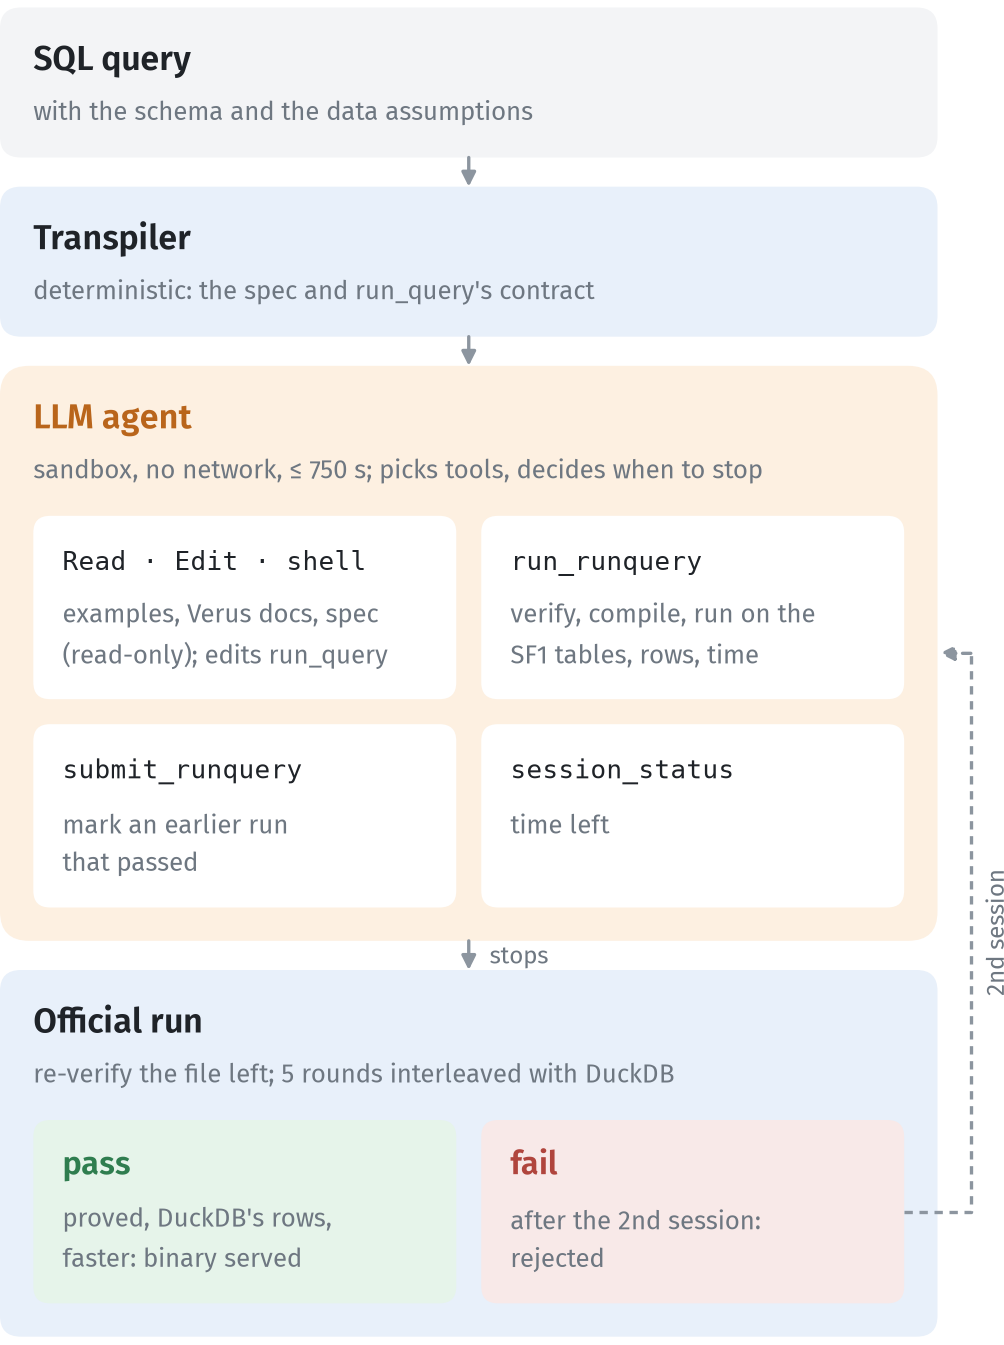
\includegraphics[keepaspectratio,alt={How one query runs: SQL query, transpiler, the LLM agent with its tools, the official run, pass or fail}]{figures/pipeline.png}}

\textbf{Steps.}

\begin{enumerate}
\def\labelenumi{\arabic{enumi}.}
\tightlist
\item
  \textbf{Transpile.} Deterministic SQL\ensuremath{\rightarrow}Verus: columnar \texttt{Cols},
  \texttt{valid\_cols} (row, cell and key bounds from the assumption
  package), and a declarative specification of the result. Schema-driven
  (no hard-coded benchmark columns, no per-query templates).
\item
  \textbf{Agent.} Writes only the \texttt{run\_query} body and its own
  helpers (proof, spec and exec functions, all verified). Host injects
  signature + \texttt{requires\ valid\_cols} + \texttt{ensures} result \ensuremath{\equiv}
  specification. Agent must not add contracts or trusted code.
\item
  \textbf{Assemble.} Single \texttt{.rs}: spec + proved body + host
  lemmas (proved) + loader + timing \texttt{main}.
\item
  \textbf{Verify.} Verus/Z3: \texttt{run\_query} meets the
  specification. Fail \ensuremath{\Rightarrow} reject (no ship).
\item
  \textbf{Compile.} \texttt{verus\ -\/-compile} \ensuremath{\rightarrow} native binary.
\item
  \textbf{Check and time.} The binary's rows are compared with DuckDB's;
  the speed verdict is the median of 5 interleaved rounds against DuckDB
  on all cores.
\item
  \textbf{Serve.} DuckDB extension caches binary; repeat queries invoke
  native path.
\end{enumerate}

\pandocbounded{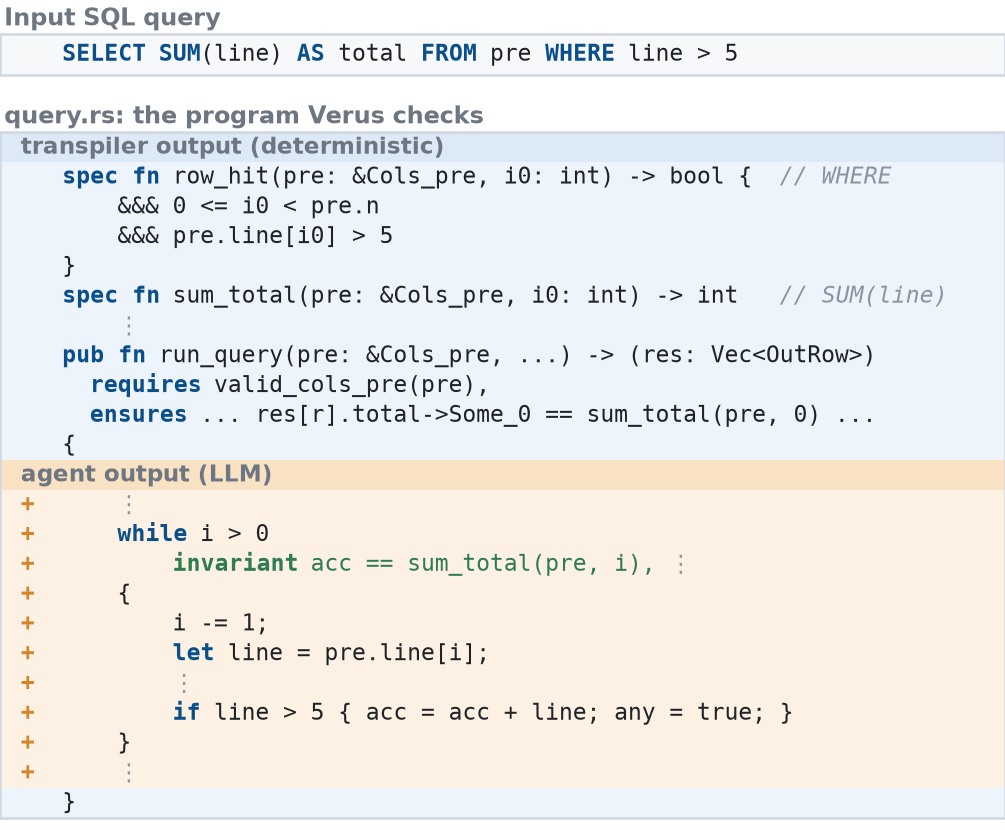
\includegraphics[keepaspectratio,alt={Worked example: the input SQL query, the transpiler's spec and contract, and the agent's run\_query body}]{figures/worked_example.png}}

\emph{Caption: A worked example. The input SQL query, and the program
Verus checks, shortened with \ensuremath{\vdots}. Blue rows are the transpiler's output
(spec and contract). Orange rows marked + are the agent's body of
\texttt{run\_query}; green text is proof annotation, erased at compile
time. The whole program is in Appendix A.}

\textbf{Trust boundary.} The assembly step makes sure the agent's code
runs only once it has been verified: the host refuses a body that uses
assume, admit or external\_body, places the body inside the
specification it emitted, and compiles only a program Verus has checked.

{\def\LTcaptype{none} % do not increment counter
\begin{longtable}[]{@{}
  >{\raggedright\arraybackslash}p{(\linewidth - 4\tabcolsep) * \real{0.3333}}
  >{\raggedright\arraybackslash}p{(\linewidth - 4\tabcolsep) * \real{0.3333}}
  >{\raggedright\arraybackslash}p{(\linewidth - 4\tabcolsep) * \real{0.3333}}@{}}
\toprule\noalign{}
\begin{minipage}[b]{\linewidth}\raggedright
What
\end{minipage} & \begin{minipage}[b]{\linewidth}\raggedright
Status
\end{minipage} & \begin{minipage}[b]{\linewidth}\raggedright
Notes
\end{minipage} \\
\midrule\noalign{}
\endhead
\bottomrule\noalign{}
\endlastfoot
Agent \texttt{run\_query} and helpers & Proved & No \texttt{assume},
\texttt{admit}, \texttt{external\_body}; admission rejects them \\
Host helper lemmas (star join, group close, distinct, folds) & Proved &
Emitted per query shape \\
Float idealization (11) + IEEE division by zero (1) & Trusted & Only for
AVG and ratios \\
Data assumptions (row/value caps, unique keys, nullability) & Checked at
load & Assumption package; \texttt{check.py} and \texttt{main} \\
Loader and timing \texttt{main} & Unverified Rust & Runtime asserts; row
check against DuckDB \\
Transpiler (SQL \ensuremath{\equiv} spec) & Tested, not proved & Differential checks
against DuckDB, adversary reviews \\
vstd, Verus, Z3, rustc & Trusted base & Thread spawn/join, Vec, Arc
specs \\
\end{longtable}
}

The data assumptions come from the user's own DuckDB: a profiling tool
measures row counts, value ranges, distinct counts and join sizes,
proposes each cap with a margin (rounded up to a power of two), and the
user approves every claim; unique keys stay proposals until the user
accepts them.

\subsection{System notes}\label{system-notes}

\subsubsection{Agent sandbox}\label{agent-sandbox}

\begin{itemize}
\tightlist
\item
  The agent (Claude Code) runs in Docker with no network except the
  model API through an allowlisted egress bridge.
\item
  It edits only marked regions; verifies and submits through MCP tools
  (\texttt{run\_runquery}, \texttt{verify\_functions} for partial
  checks, \texttt{submit\_runquery}).
\item
  Examples mode: \texttt{full}, \texttt{principles} (7 technique
  examples on made-up tables), \texttt{none} (task, rules, tools, Verus
  reference docs only).
\item
  Optional data profile: exact SQL statistics per query (row counts,
  selectivities, group counts), no query plan.
\end{itemize}

\subsubsection{SQL surface}\label{sql-surface}

\begin{itemize}
\tightlist
\item
  Supported: joins (incl.~comma joins, star joins on unique keys),
  filters, GROUP BY/HAVING, ORDER BY/LIMIT, SUM/COUNT/MIN/MAX/AVG, COUNT
  DISTINCT, uncorrelated scalar subqueries, anti-joins, NULLs, DECIMAL,
  DATE, dictionary strings.
\item
  Not supported: recursion, window functions, outer joins (except
  anti-join), set operations, string functions, correlated subqueries;
  5+ table joins lightly tested.
\item
  Workloads: TPC-H SF1 and SSB SF1.
\end{itemize}

\subsection{Evaluation}\label{evaluation}

With Claude Opus 5.5 and no worked examples, all five queries run so far
proved, returned DuckDB's rows and beat all-core DuckDB, by 1.60\ensuremath{\times} to
5.20\ensuremath{\times} (median 2.42\ensuremath{\times}). The other 14 queries are still to run. Per-query
results, configuration and cost are in Appendix F.

\pandocbounded{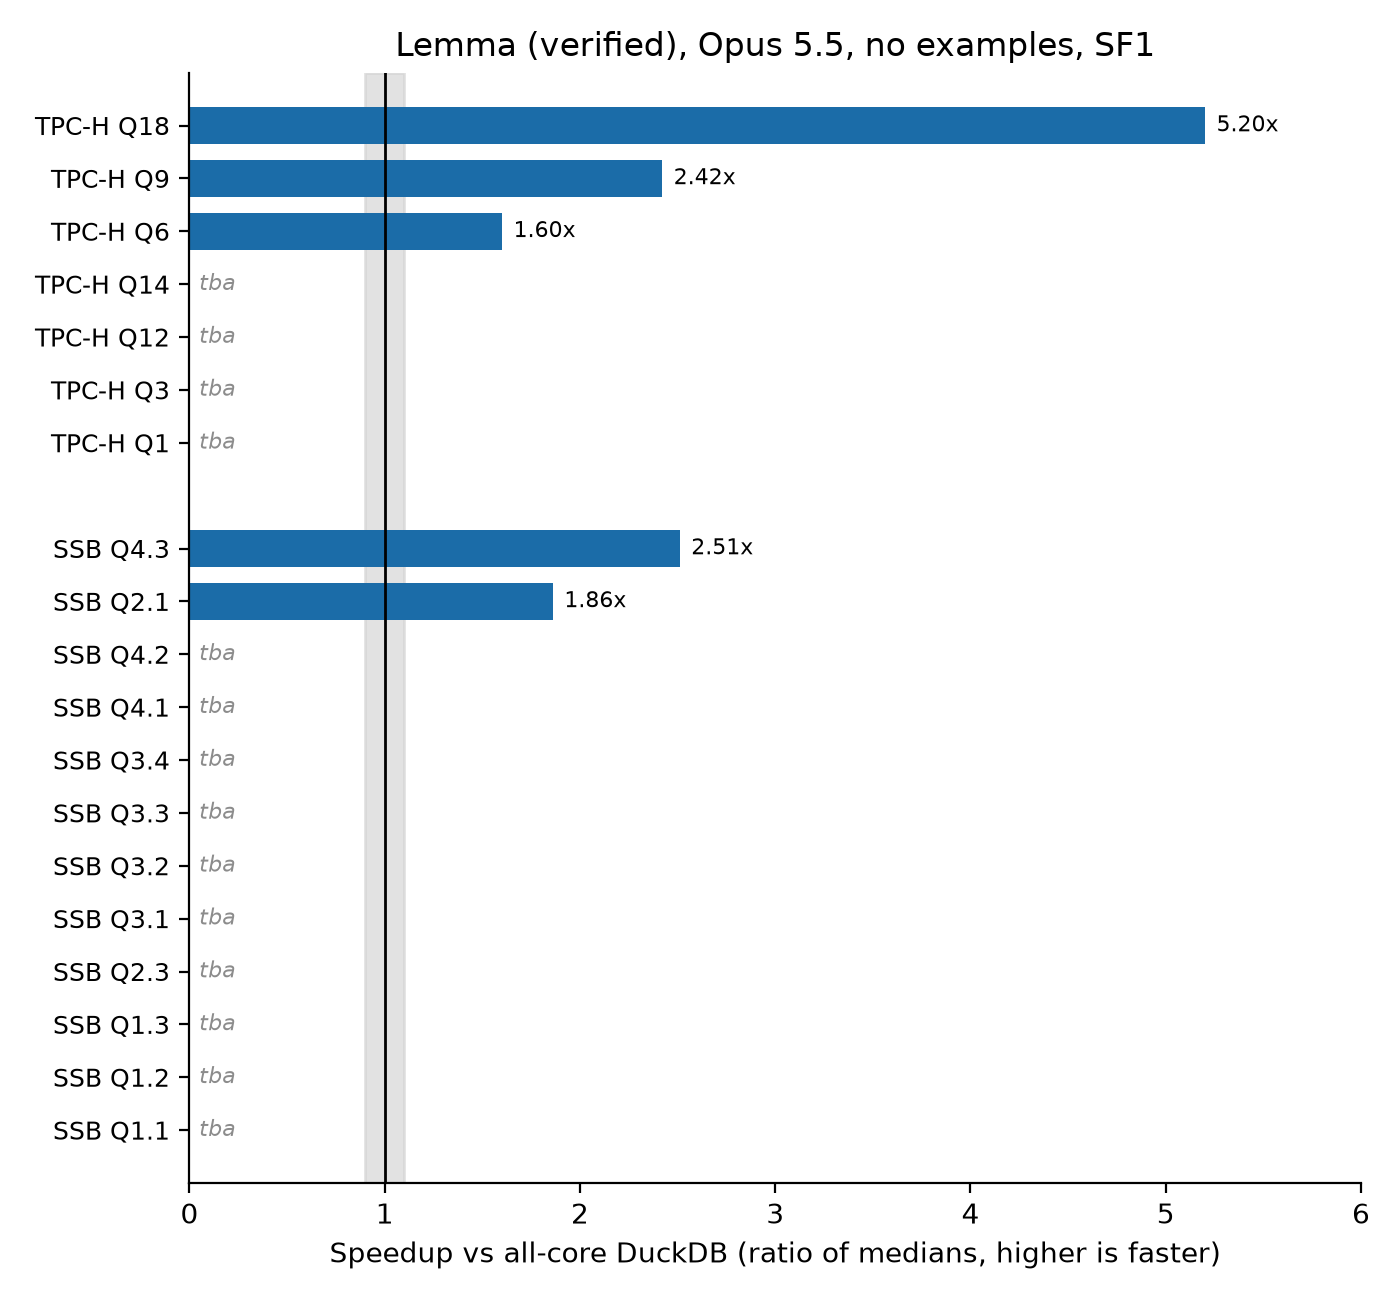
\includegraphics[keepaspectratio,alt={Speedup over all-core DuckDB per query, SF1: Opus 5.5 without worked examples; tba = not yet run in this configuration}]{figures/speedup.png}}

\emph{Figure: speedup over all-core DuckDB at SF1, Claude Opus 5.5
without worked examples (Appendix F). tba = not yet run in this
configuration.}

\textbf{Setup.} Claude Opus 5.5 in the container, no worked examples, a
data profile of SQL statistics, at most 2 \ensuremath{\times} 30 min of agent time and
\$20 per query; dictionary strings, star-join specs. Official verdict:
hot runs, median of 5 interleaved rounds against DuckDB 1.5.4 on all 8
threads, 8 GB memory limit. AMD Ryzen AI 5 330 (4 cores / 8 threads), 14
GB RAM. SF1.

\textbf{Number formats.} Both Lemma and DuckDB represent
\texttt{DECIMAL} and \texttt{DATE} values as exact integers; floating
point appears only where SQL returns \texttt{DOUBLE} (\texttt{AVG} in
TPC-H Q1 and the ratio in Q14), where both compute in IEEE double and
our specification treats the operations as exact reals (see Trust
boundary).

GenDB's times come from different hardware (SF10, 32 cores, 384 GB), so
we compare only ratios to DuckDB on the same machine.

An earlier run with Claude Sonnet 5.5 and full worked examples proved
all 19 queries (median 2.04\ensuremath{\times} on SSB, 1.29\ensuremath{\times} on TPC-H), but its examples
included the solutions of 6 of those queries, so it does not measure
generalization.

\subsection{Related work}\label{related-work}

\textbf{LLM-synthesized query engines.}

\begin{itemize}
\tightlist
\item
  \textbf{CodexDB} {[}Trummer2022CodexDB{]}: LLM synthesizes per-query
  processing code from SQL (+ NL instructions); correctness via tests /
  execution, not formal proof vs a MethodSpec.
\item
  \textbf{GPT-DB} {[}Trummer2023GPTDB{]}: follow-on demo; customizable
  GPT-generated SQL processing code.
\item
  \textbf{GenDB} {[}Lao2026GenDB{]}: multi-agent instance-optimized C++
  per query (workload / storage / plan / codegen / optimize); strong
  speedups vs DuckDB/Umbra; correctness mainly empirical / inspection.
\item
  \textbf{Bespoke OLAP} {[}Wehrstein2026Bespoke{]}: full
  workload-specific C++ engine (storage + executors) with iterative perf
  feedback; validates vs DuckDB, not formal refinement.
\end{itemize}

\textbf{Classical query compilation (not LLM).}

\begin{itemize}
\tightlist
\item
  \textbf{HIQUE} {[}Krikellas2010HIQUE{]}: template-based holistic
  per-query C codegen.
\item
  \textbf{HyPer} {[}Neumann2011Hyper{]} / adaptive execution
  {[}Kohn2018Adaptive{]}: data-centric LLVM compilation;
  interpret\ensuremath{\leftrightarrow}compile switching.
\item
  \textbf{LegoBase} {[}Klonatos2014LegoBase{]}: generative programming /
  staging; Scala\ensuremath{\rightarrow}specialized C.
\item
  \textbf{Umbra} {[}Kersten2021UmbraFlyingStart{]}: fast compile (Flying
  Start) + optimizing LLVM path.
\item
  \textbf{NoisePage / Peloton line} {[}Menon2017Relaxed,
  Menon2020Permutable{]}: relaxed operator fusion; permutable compiled
  queries without full recompile.
\item
  \textbf{DBToaster} {[}Ahmad2012DBToaster{]}, \textbf{Tupleware}
  {[}Crotty2015Tupleware{]}, \textbf{Weld} {[}Palkar2018Weld{]}:
  specialized / IR-based codegen lineages (cite selectively).
\end{itemize}

\textbf{Formal SQL semantics \& verified query compilers. TODO PRUNE,
NOT SO INTERESTEING}

\begin{itemize}
\tightlist
\item
  \textbf{HoTTSQL} {[}Chu2017HoTTSQL{]}: mechanized denotational SQL
  semantics (Coq); prove rewrite rules.
\item
  \textbf{Cosette} {[}Chu2017Cosette{]}: automated SQL equivalence
  prover (proof or counterexample).
\item
  \textbf{SQL\_Coq / SQL algebra} {[}Benzaken2019SQLCoq{]}: Coq
  semantics for realistic SQL + algebra equivalence.
\item
  \textbf{Physical algebra / QEP layer} {[}Benzaken2018Physical{]}: Coq
  formalization of low-level RDBMS operators / physical plans.
\item
  \textbf{Q*cert} {[}Auerbach2017Qcert{]}: Coq platform for verified
  query compilation (NRA\^{}e, multi-target).
\item
  \textbf{DBCert} {[}Benzaken2022DBCert{]}: verified SQL\_Coq \ensuremath{\rightarrow} Imp
  (then JS); correct-by-construction compiler, \emph{not} LLM-written
  hot paths.
\item
  Contrast w/ Lemma: those systems verify a \emph{fixed} compiler or
  rewrite; Lemma verifies an \emph{LLM-written} executor against a
  transpiled MethodSpec.
\end{itemize}

\textbf{LLM + machine-checked code (general, not DB-specific).}

\begin{itemize}
\tightlist
\item
  \textbf{AlphaVerus} {[}Aggarwal2025AlphaVerus{]}: LLM\ensuremath{\rightarrow}verified Verus
  via translation + verifier-guided tree search (``Treefinement'').
\item
  \textbf{Vericoding benchmarks} {[}Dougherty2025Vericoding{]}: large
  Dafny/Verus/Lean specs for LLM verified synthesis eval.
\item
  Related: Formal Disco / verified-program datasets; DafnyBench-style
  eval --- cite if space.
\end{itemize}

\textbf{Adjacent LLM\ensuremath{\times}DB (not executor synthesis).}

\begin{itemize}
\tightlist
\item
  \textbf{SQLBarber} {[}Lao2025SQLBarber{]}: LLM generates customized
  SQL \emph{workloads} / templates (benchmarking), not query executors.
\item
  Text-to-SQL / NL\ensuremath{\rightarrow}SQL systems: large literature; orthogonal (query
  \emph{text}, not verified runtime).
\end{itemize}

\textbf{Verification substrate.}

\begin{itemize}
\tightlist
\item
  \textbf{Verus} {[}Lattuada2023Verus{]}: SMT verification for Rust;
  Lemma's proof target.
\item
  \textbf{Dafny} {[}Leino2010Dafny{]}: prior Lemma path; same
  agent-vs-spec idea, heavier codegen/postprocess story.
\end{itemize}

\textbf{Positioning (one line).}

\begin{itemize}
\tightlist
\item
  Lemma \ensuremath{\approx} GenDB/CodexDB-style synthesis \emph{plus} DBCert/Cosette-style
  machine-checked guarantees, scoped to \texttt{run\_query} \ensuremath{\equiv} MethodSpec
  before ship.
\end{itemize}

\subsection{Future work}\label{future-work}

\begin{enumerate}
\def\labelenumi{\arabic{enumi}.}
\tightlist
\item
  Shrink TRUSTED surface: exact AVG and division as integer fractions
  (removes the 12 float items for DECIMAL data); verify the loader's
  runtime checks.
\item
  Stronger optimizing harness / ``RSI''-style self-improvement loop
  (cite recent RSI harness papers --- TODO).
\item
  Improve extension sandbox; optional Inspect-style pluggable agent CLI
  bridge.
\end{enumerate}

Ablation studies / feature additions:

\begin{itemize}
\tightlist
\item
  giving pre-made recipes
\item
  adding float-trusteds
\item
  removing/adding trusteds

  \begin{itemize}
  \tightlist
  \item
    Most recently (11 oct) we are using vstd trusteds
  \end{itemize}
\item
  weaker/stronger model
\item
  use ``imperative'', not ``declarative'' specs
\item
  on some novel set of queries: allow internet access
\end{itemize}

It is unclear where the current system is superior to duckdb. A hot run
is faster than DuckDB, but loading in data and running it is
(supposedly) not. The current simple load-cols-as-vectors-into-RAM
format is also (arguably) not as production-ready as DuckDB's or that of
other trad. DBs in different aspects, because it e.g.~does not paginate
or compress. A plan for making a system that is actually competitive in
the real world would be to make it operate on the data structure of an
established DB. This would also allow for running it generatively or
with trad. DB engine, depending on current need.

\subsection{References}\label{references}

\begin{itemize}
\tightlist
\item
  {[}Trummer2022CodexDB{]} Immanuel Trummer. CodexDB: Synthesizing Code
  for Query Processing from Natural Language Instructions using GPT-3
  Codex. \emph{PVLDB}, 15(11):2921--2928, 2022.
\item
  {[}Trummer2023GPTDB{]} Immanuel Trummer. Demonstrating GPT-DB:
  Generating Query-Specific and Customizable Code for SQL Processing
  with GPT-4. \emph{PVLDB}, 16(12), 2023.
\item
  {[}Lao2026GenDB{]} Jiale Lao and Immanuel Trummer. GenDB: The Next
  Generation of Query Processing -- Synthesized, Not Engineered.
  arXiv:2603.02081, 2026.
\item
  {[}Wehrstein2026Bespoke{]} Johannes Wehrstein, Timo Eckmann, Matthias
  Jasny, and Carsten Binnig. Bespoke OLAP: Synthesizing
  Workload-Specific One-size-fits-one Database Engines.
  arXiv:2603.02001, 2026.
\item
  {[}Krikellas2010HIQUE{]} Konstantinos Krikellas, Stratis D. Viglas,
  and Marcelo Cintra. Generating Code for Holistic Query Evaluation. In
  \emph{ICDE}, 2010.
\item
  {[}Neumann2011Hyper{]} Thomas Neumann. Efficiently Compiling Efficient
  Query Plans for Modern Hardware. \emph{PVLDB}, 4(9):539--550, 2011.
\item
  {[}Kohn2018Adaptive{]} André Kohn, Viktor Leis, and Thomas Neumann.
  Adaptive Execution of Compiled Queries. In \emph{ICDE}, 2018.
\item
  {[}Klonatos2014LegoBase{]} Yannis Klonatos, Christoph Koch, Tiark
  Rompf, and Hassan Chafi. Building Efficient Query Engines in a
  High-Level Language. \emph{PVLDB}, 7(10):853--864, 2014.
\item
  {[}Kersten2021UmbraFlyingStart{]} Timo Kersten, Viktor Leis, and
  Thomas Neumann. Tidy Tuples and Flying Start: Fast Compilation and
  Fast Execution of Relational Queries in Umbra. \emph{VLDB J.}, 2021.
\item
  {[}Menon2017Relaxed{]} Prashanth Menon, Todd C. Mowry, and Andrew
  Pavlo. Relaxed Operator Fusion for In-Memory Databases: Making
  Compilation, Vectorization, and Prefetching Work Together At Last.
  \emph{PVLDB}, 11(1):1--13, 2017.
\item
  {[}Menon2020Permutable{]} Prashanth Menon, Amadou Ngom, Lin Ma, Todd
  C. Mowry, and Andrew Pavlo. Permutable Compiled Queries: Dynamically
  Adapting Compiled Queries without Recompiling. \emph{PVLDB},
  14(2):101--113, 2020.
\item
  {[}Ahmad2012DBToaster{]} Yanif Ahmad, Oliver Kennedy, Christoph Koch,
  and Milos Nikolic. DBToaster: Higher-order Delta Processing for
  Dynamic, Frequently Fresh Views. \emph{PVLDB}, 5(10):968--979, 2012.
  (confirm exact citation if needed)
\item
  {[}Crotty2015Tupleware{]} Andrew Crotty, Alex Galakatos, Kayhan
  Dursun, Tim Kraska, Carsten Binnig, Ugur Cetintemel, and Stan Zdonik.
  An Architecture for Compiling UDF-centric Workflows. \emph{PVLDB},
  8(12):1466--1477, 2015. (Tupleware lineage; confirm title/pages)
\item
  {[}Palkar2018Weld{]} Shoumik Palkar, James Thomas, Deepak Narayanan,
  Pratiksha Thaker, Rahul Palamuttam, Parimajan Negi, Anil Shanbhag,
  Malte Schwarzkopf, Holger Pirk, Saman Amarasinghe, Samuel Madden, and
  Matei Zaharia. Evaluating End-to-End Optimization for Data Analytics
  Applications in Weld. \emph{PVLDB}, 11(9):1002--1015, 2018.
\item
  {[}Chu2017HoTTSQL{]} Shumo Chu, Konstantin Weitz, Alvin Cheung, and
  Dan Suciu. HoTTSQL: Proving Query Rewrites with Univalent SQL
  Semantics. In \emph{PLDI}, 2017.
\item
  {[}Chu2017Cosette{]} Shumo Chu, Chenglong Wang, Konstantin Weitz, and
  Alvin Cheung. Cosette: An Automated Prover for SQL. In \emph{CIDR},
  2017.
\item
  {[}Benzaken2019SQLCoq{]} Véronique Benzaken and Évelyne Contejean. A
  Coq Mechanised Formal Semantics for Realistic SQL Queries: Formally
  Reconciling SQL and Relational Algebra. In \emph{CPP}, 2019. (confirm
  venue (CPP / related))
\item
  {[}Benzaken2018Physical{]} Véronique Benzaken, Évelyne Contejean,
  Chantal Keller, and Eunice Martins. A Coq Formalisation of SQL's
  Execution Engines. (ITP / related --- polish venue) 2018.
\item
  {[}Auerbach2017Qcert{]} Joshua S. Auerbach, Martin Hirzel, Louis
  Mandel, Avraham Shinnar, and Jérôme Siméon. Q*cert: A Platform for
  Implementing and Verifying Query Compilers. In \emph{SIGMOD} (demo),
  2017.
\item
  {[}Benzaken2022DBCert{]} Véronique Benzaken, Évelyne Contejean,
  Mohammed Houssem Hachmaoui, Chantal Keller, Louis Mandel, Avraham
  Shinnar, and Jérôme Siméon. Translating Canonical SQL to Imperative
  Code in Coq. \emph{Proc. ACM Program. Lang.}, 6(OOPSLA1), 2022.
\item
  {[}Aggarwal2025AlphaVerus{]} Pranjal Aggarwal, Bryan Parno, and Sean
  Welleck. AlphaVerus: Bootstrapping Formally Verified Code Generation
  through Self-Improving Translation and Treefinement. In \emph{ICML},
  2025.
\item
  {[}Dougherty2025Vericoding{]} Sergiu Bursuc, Theodore Ehrenborg,
  Shaowei Lin, Lacramioara Astefanoaei, Ionel Emilian Chiosa, Jure
  Kukovec, Alok Singh, Oliver Butterley, Adem Bizid, Quinn Dougherty,
  Miranda Zhao, Max Tan, and Max Tegmark. A Benchmark for Vericoding:
  Formally Verified Program Synthesis. arXiv:2509.22908, 2025.
\item
  {[}Lao2025SQLBarber{]} Jiale Lao and Immanuel Trummer. SQLBarber: A
  System Leveraging Large Language Models to Generate Customized and
  Realistic SQL Workloads. arXiv:2507.06192, 2025.
\item
  {[}Lattuada2023Verus{]} Andrea Lattuada, Travis Hance, Chanhee Cho,
  Matthias Brun, Isitha Subasinghe, Yi Zhou, Jon Howell, Bryan Parno,
  and Chris Hawblitzel. Verus: Verifying Rust Programs using Linear
  Ghost Types. \emph{Proc. ACM Program. Lang.}, 7(OOPSLA1), 2023.
\item
  {[}Leino2010Dafny{]} K. Rustan M. Leino. Dafny: An Automatic Program
  Verifier for Functional Correctness. In \emph{LPAR}, 2010.
\end{itemize}

\subsection{Acknowledgements}\label{acknowledgements}

TODO.

\subsection{Appendix A: Full program for one
query}\label{appendix-a-full-program-for-one-query}

The whole program Verus checks for
\texttt{SELECT\ SUM(line)\ AS\ total\ FROM\ pre\ WHERE\ line\ \textgreater{}\ 5},
verbatim except the 79 \texttt{use\ vstd::...} lines. Listing A.1 is the
transpiler's output: the data assumptions (\texttt{valid\_cols\_pre}),
the WHERE clause (\texttt{row\_hit}), \texttt{SUM} as a recursive fold,
and the contract of \texttt{run\_query}. Listing A.2 is the agent's body
of \texttt{run\_query}, which goes between the \texttt{AGENT\_EDIT}
markers (the end marker and two closing braces follow it). The body is
\texttt{tests/fixtures/declarative\_proofs/ungrouped\_sum\_where.rs} in
\href{https://github.com/emilschmitz/lemma}{github.com/emilschmitz/lemma};
the test suite verifies the assembled program with Verus.

\emph{Listing A.1: Transpiler output (deterministic).}

\begin{Shaded}
\begin{Highlighting}[]
\PreprocessorTok{verus!} \OperatorTok{\{}

\KeywordTok{pub} \KeywordTok{const}\NormalTok{ ROW\_CAP\_pre}\OperatorTok{:} \DataTypeTok{usize} \OperatorTok{=} \DecValTok{64}\OperatorTok{;}
\KeywordTok{pub} \KeywordTok{struct}\NormalTok{ Cols\_pre }\OperatorTok{\{}
    \KeywordTok{pub}\NormalTok{ n}\OperatorTok{:} \DataTypeTok{usize}\OperatorTok{,}
    \KeywordTok{pub}\NormalTok{ line}\OperatorTok{:} \DataTypeTok{Vec}\OperatorTok{\textless{}}\DataTypeTok{i64}\OperatorTok{\textgreater{},}
\OperatorTok{\}}

\KeywordTok{pub}\NormalTok{ open spec }\KeywordTok{fn}\NormalTok{ valid\_cols\_pre(pre}\OperatorTok{:} \OperatorTok{\&}\NormalTok{Cols\_pre) }\OperatorTok{{-}\textgreater{}} \DataTypeTok{bool} \OperatorTok{\{}
    \OperatorTok{\&\&\&}\NormalTok{ pre}\OperatorTok{.}\NormalTok{line}\OperatorTok{@.}\NormalTok{len() }\OperatorTok{==}\NormalTok{ pre}\OperatorTok{.}\NormalTok{n }\KeywordTok{as}\NormalTok{ int}
    \OperatorTok{\&\&\&}\NormalTok{ pre}\OperatorTok{.}\NormalTok{n }\KeywordTok{as}\NormalTok{ int }\OperatorTok{\textless{}=}\NormalTok{ ROW\_CAP\_pre }\KeywordTok{as}\NormalTok{ int}
\OperatorTok{\}}

\KeywordTok{pub}\NormalTok{ open spec }\KeywordTok{fn}\NormalTok{ row\_hit(pre}\OperatorTok{:} \OperatorTok{\&}\NormalTok{Cols\_pre}\OperatorTok{,}\NormalTok{ i0}\OperatorTok{:}\NormalTok{ int) }\OperatorTok{{-}\textgreater{}} \DataTypeTok{bool} \OperatorTok{\{}
    \OperatorTok{\&\&\&} \DecValTok{0} \OperatorTok{\textless{}=}\NormalTok{ i0 }\OperatorTok{\textless{}}\NormalTok{ pre}\OperatorTok{.}\NormalTok{n }\KeywordTok{as}\NormalTok{ int}
    \OperatorTok{\&\&\&}\NormalTok{ (((pre}\OperatorTok{.}\NormalTok{line}\OperatorTok{@}\NormalTok{[i0] }\KeywordTok{as}\NormalTok{ int) }\OperatorTok{\textgreater{}} \DecValTok{5}\NormalTok{))}
\OperatorTok{\}}

\KeywordTok{pub}\NormalTok{ open spec }\KeywordTok{fn}\NormalTok{ sum\_total\_val(pre}\OperatorTok{:} \OperatorTok{\&}\NormalTok{Cols\_pre}\OperatorTok{,}\NormalTok{ i0}\OperatorTok{:}\NormalTok{ int) }\OperatorTok{{-}\textgreater{}}\NormalTok{ int }\OperatorTok{\{}
    \ControlFlowTok{if} \DecValTok{0} \OperatorTok{\textless{}=}\NormalTok{ i0 }\OperatorTok{\textless{}}\NormalTok{ pre}\OperatorTok{.}\NormalTok{n }\KeywordTok{as}\NormalTok{ int }\OperatorTok{\{}
\NormalTok{        (pre}\OperatorTok{.}\NormalTok{line}\OperatorTok{@}\NormalTok{[i0] }\KeywordTok{as}\NormalTok{ int)}
    \OperatorTok{\}} \ControlFlowTok{else} \OperatorTok{\{}
\NormalTok{        0int}
    \OperatorTok{\}}
\OperatorTok{\}}

\KeywordTok{pub}\NormalTok{ open spec }\KeywordTok{fn}\NormalTok{ sum\_total(pre}\OperatorTok{:} \OperatorTok{\&}\NormalTok{Cols\_pre}\OperatorTok{,}\NormalTok{ i0}\OperatorTok{:}\NormalTok{ int) }\OperatorTok{{-}\textgreater{}}\NormalTok{ int}
\NormalTok{    decreases pre}\OperatorTok{.}\NormalTok{n }\KeywordTok{as}\NormalTok{ int }\OperatorTok{{-}}\NormalTok{ i0}
\OperatorTok{\{}
    \ControlFlowTok{if}\NormalTok{ i0 }\OperatorTok{\textless{}} \DecValTok{0} \OperatorTok{||}\NormalTok{ i0 }\OperatorTok{\textgreater{}=}\NormalTok{ pre}\OperatorTok{.}\NormalTok{n }\KeywordTok{as}\NormalTok{ int }\OperatorTok{\{}
\NormalTok{        0int}
    \OperatorTok{\}} \ControlFlowTok{else} \OperatorTok{\{}
\NormalTok{        (}\ControlFlowTok{if}\NormalTok{ row\_hit(pre}\OperatorTok{,}\NormalTok{ i0) }\OperatorTok{\{}\NormalTok{ sum\_total\_val(pre}\OperatorTok{,}\NormalTok{ i0) }\OperatorTok{\}} \ControlFlowTok{else} \OperatorTok{\{}\NormalTok{ 0int }\OperatorTok{\}}\NormalTok{) }\OperatorTok{+}\NormalTok{ sum\_total(pre}\OperatorTok{,}\NormalTok{ i0 }\OperatorTok{+} \DecValTok{1}\NormalTok{)}
    \OperatorTok{\}}
\OperatorTok{\}}

\CommentTok{// HOST\_LEMMAS\_START}

\CommentTok{// HOST\_LEMMAS\_}\RegionMarkerTok{END}

\KeywordTok{pub} \KeywordTok{struct}\NormalTok{ OutRow }\OperatorTok{\{}
    \KeywordTok{pub}\NormalTok{ total}\OperatorTok{:} \DataTypeTok{Option}\OperatorTok{\textless{}}\DataTypeTok{i128}\OperatorTok{\textgreater{},}
\OperatorTok{\}}

\CommentTok{// AGENT\_HELPERS\_START}
\CommentTok{// AGENT\_HELPERS\_}\RegionMarkerTok{END}
\KeywordTok{pub} \KeywordTok{fn}\NormalTok{ run\_query(pre}\OperatorTok{:} \OperatorTok{\&}\NormalTok{Cols\_pre}\OperatorTok{,}\NormalTok{ pre\_arc}\OperatorTok{:} \OperatorTok{\&}\PreprocessorTok{std::sync::}\NormalTok{Arc}\OperatorTok{\textless{}}\NormalTok{Cols\_pre}\OperatorTok{\textgreater{}}\NormalTok{) }\OperatorTok{{-}\textgreater{}}\NormalTok{ (res}\OperatorTok{:} \DataTypeTok{Vec}\OperatorTok{\textless{}}\NormalTok{OutRow}\OperatorTok{\textgreater{}}\NormalTok{)}
\NormalTok{    requires}
        \OperatorTok{**}\NormalTok{pre\_arc }\OperatorTok{==} \OperatorTok{*}\NormalTok{pre}\OperatorTok{,}
\NormalTok{        valid\_cols\_pre(pre)}\OperatorTok{,}
\NormalTok{    ensures}
\NormalTok{        (((}\ConstantTok{true}\NormalTok{) }\OperatorTok{\&\&}\NormalTok{ res}\OperatorTok{@.}\NormalTok{len() }\OperatorTok{==} \DecValTok{1} \OperatorTok{\&\&}\NormalTok{ (forall}\OperatorTok{|}\NormalTok{r}\OperatorTok{:}\NormalTok{ int}\OperatorTok{|} \AttributeTok{\#![}\NormalTok{trigger res}\OperatorTok{@}\NormalTok{[r}\AttributeTok{]}\NormalTok{] }\DecValTok{0} \OperatorTok{\textless{}=}\NormalTok{ r }\OperatorTok{\textless{}}\NormalTok{ res}\OperatorTok{@.}\NormalTok{len() }\OperatorTok{==\textgreater{}}\NormalTok{ (((exists}\OperatorTok{|}\NormalTok{i0}\OperatorTok{:}\NormalTok{ int}\OperatorTok{|} \AttributeTok{\#![}\NormalTok{trigger row\_hit}\AttributeTok{(}\NormalTok{pre}\OperatorTok{,}\NormalTok{ i0}\AttributeTok{)]}\NormalTok{ row\_hit(pre}\OperatorTok{,}\NormalTok{ i0)) }\OperatorTok{==\textgreater{}}\NormalTok{ ((res}\OperatorTok{@}\NormalTok{[r]}\OperatorTok{.}\NormalTok{total is }\ConstantTok{Some}\NormalTok{) }\OperatorTok{\&\&}\NormalTok{ (res}\OperatorTok{@}\NormalTok{[r]}\OperatorTok{.}\NormalTok{total}\OperatorTok{{-}\textgreater{}}\NormalTok{Some\_0 }\KeywordTok{as}\NormalTok{ int) }\OperatorTok{==}\NormalTok{ sum\_total(pre}\OperatorTok{,} \DecValTok{0}\NormalTok{))) }\OperatorTok{\&\&}\NormalTok{ (}\OperatorTok{!}\NormalTok{(exists}\OperatorTok{|}\NormalTok{i0}\OperatorTok{:}\NormalTok{ int}\OperatorTok{|} \AttributeTok{\#![}\NormalTok{trigger row\_hit}\AttributeTok{(}\NormalTok{pre}\OperatorTok{,}\NormalTok{ i0}\AttributeTok{)]}\NormalTok{ row\_hit(pre}\OperatorTok{,}\NormalTok{ i0)) }\OperatorTok{==\textgreater{}}\NormalTok{ (res}\OperatorTok{@}\NormalTok{[r]}\OperatorTok{.}\NormalTok{total is }\ConstantTok{None}\NormalTok{))))) }\OperatorTok{||}\NormalTok{ (}\OperatorTok{!}\NormalTok{(}\ConstantTok{true}\NormalTok{) }\OperatorTok{\&\&}\NormalTok{ res}\OperatorTok{@.}\NormalTok{len() }\OperatorTok{==} \DecValTok{0}\NormalTok{))}\OperatorTok{,}
\OperatorTok{\{}
\CommentTok{// AGENT\_EDIT\_START}
\end{Highlighting}
\end{Shaded}

\emph{Listing A.2: The agent's body of \texttt{run\_query}.}

\begin{Shaded}
\begin{Highlighting}[]
    \KeywordTok{let} \KeywordTok{mut}\NormalTok{ acc}\OperatorTok{:} \DataTypeTok{i128} \OperatorTok{=} \DecValTok{0}\OperatorTok{;}
    \KeywordTok{let} \KeywordTok{mut}\NormalTok{ any}\OperatorTok{:} \DataTypeTok{bool} \OperatorTok{=} \ConstantTok{false}\OperatorTok{;}
    \KeywordTok{let} \KeywordTok{mut}\NormalTok{ i}\OperatorTok{:} \DataTypeTok{usize} \OperatorTok{=}\NormalTok{ pre}\OperatorTok{.}\NormalTok{n}\OperatorTok{;}
    \ControlFlowTok{while}\NormalTok{ i }\OperatorTok{\textgreater{}} \DecValTok{0}
\NormalTok{        invariant}
\NormalTok{            i }\OperatorTok{\textless{}=}\NormalTok{ pre}\OperatorTok{.}\NormalTok{n}\OperatorTok{,}
\NormalTok{            valid\_cols\_pre(pre)}\OperatorTok{,}
\NormalTok{            acc }\KeywordTok{as}\NormalTok{ int }\OperatorTok{==}\NormalTok{ sum\_total(pre}\OperatorTok{,}\NormalTok{ i }\KeywordTok{as}\NormalTok{ int)}\OperatorTok{,}
            \OperatorTok{{-}}\NormalTok{((pre}\OperatorTok{.}\NormalTok{n }\OperatorTok{{-}}\NormalTok{ i) }\KeywordTok{as}\NormalTok{ int) }\OperatorTok{*} \ErrorTok{0x8000\_0000\_0000\_0000int} \OperatorTok{\textless{}=}\NormalTok{ acc }\KeywordTok{as}\NormalTok{ int}\OperatorTok{,}
\NormalTok{            acc }\KeywordTok{as}\NormalTok{ int }\OperatorTok{\textless{}=}\NormalTok{ ((pre}\OperatorTok{.}\NormalTok{n }\OperatorTok{{-}}\NormalTok{ i) }\KeywordTok{as}\NormalTok{ int) }\OperatorTok{*} \ErrorTok{0x8000\_0000\_0000\_0000int}\OperatorTok{,}
\NormalTok{            any }\OperatorTok{\textless{}==\textgreater{}}\NormalTok{ exists}\OperatorTok{|}\NormalTok{i0}\OperatorTok{:}\NormalTok{ int}\OperatorTok{|} \AttributeTok{\#![}\NormalTok{trigger row\_hit}\AttributeTok{(}\NormalTok{pre}\OperatorTok{,}\NormalTok{ i0}\AttributeTok{)]}\NormalTok{ i }\KeywordTok{as}\NormalTok{ int }\OperatorTok{\textless{}=}\NormalTok{ i0 }\OperatorTok{\&\&}\NormalTok{ row\_hit(pre}\OperatorTok{,}\NormalTok{ i0)}\OperatorTok{,}
\NormalTok{        decreases i}\OperatorTok{,}
    \OperatorTok{\{}
\NormalTok{        i }\OperatorTok{{-}=} \DecValTok{1}\OperatorTok{;}
        \KeywordTok{let}\NormalTok{ line }\OperatorTok{=}\NormalTok{ pre}\OperatorTok{.}\NormalTok{line[i]}\OperatorTok{;}
\NormalTok{        proof }\OperatorTok{\{}
\NormalTok{            assert(pre}\OperatorTok{.}\NormalTok{line}\OperatorTok{@.}\NormalTok{len() }\OperatorTok{==}\NormalTok{ pre}\OperatorTok{.}\NormalTok{n }\KeywordTok{as}\NormalTok{ int)}\OperatorTok{;}
\NormalTok{            assert(row\_hit(pre}\OperatorTok{,}\NormalTok{ i }\KeywordTok{as}\NormalTok{ int) }\OperatorTok{\textless{}==\textgreater{}}\NormalTok{ ((line }\KeywordTok{as}\NormalTok{ int) }\OperatorTok{\textgreater{}} \DecValTok{5}\NormalTok{))}\OperatorTok{;}
\NormalTok{            assert(sum\_total\_val(pre}\OperatorTok{,}\NormalTok{ i }\KeywordTok{as}\NormalTok{ int) }\OperatorTok{==}\NormalTok{ line }\KeywordTok{as}\NormalTok{ int)}\OperatorTok{;}
\NormalTok{            reveal\_with\_fuel(sum\_total}\OperatorTok{,} \DecValTok{2}\NormalTok{)}\OperatorTok{;}
        \OperatorTok{\}}
        \ControlFlowTok{if}\NormalTok{ line }\OperatorTok{\textgreater{}} \DecValTok{5} \OperatorTok{\{}
\NormalTok{            acc }\OperatorTok{=}\NormalTok{ acc }\OperatorTok{+}\NormalTok{ (line }\KeywordTok{as} \DataTypeTok{i128}\NormalTok{)}\OperatorTok{;}
\NormalTok{            any }\OperatorTok{=} \ConstantTok{true}\OperatorTok{;}
\NormalTok{            proof }\OperatorTok{\{}
\NormalTok{                assert(row\_hit(pre}\OperatorTok{,}\NormalTok{ i }\KeywordTok{as}\NormalTok{ int))}\OperatorTok{;}
            \OperatorTok{\}}
        \OperatorTok{\}}
    \OperatorTok{\}}
    \KeywordTok{let} \KeywordTok{mut}\NormalTok{ res}\OperatorTok{:} \DataTypeTok{Vec}\OperatorTok{\textless{}}\NormalTok{OutRow}\OperatorTok{\textgreater{}} \OperatorTok{=} \DataTypeTok{Vec}\PreprocessorTok{::}\NormalTok{new()}\OperatorTok{;}
\NormalTok{    res}\OperatorTok{.}\NormalTok{push(OutRow }\OperatorTok{\{}\NormalTok{ total}\OperatorTok{:} \ControlFlowTok{if}\NormalTok{ any }\OperatorTok{\{} \ConstantTok{Some}\NormalTok{(acc) }\OperatorTok{\}} \ControlFlowTok{else} \OperatorTok{\{} \ConstantTok{None} \OperatorTok{\}} \OperatorTok{\}}\NormalTok{)}\OperatorTok{;}
\NormalTok{    proof }\OperatorTok{\{}
\NormalTok{        assert(res}\OperatorTok{@}\NormalTok{[}\DecValTok{0}\NormalTok{]}\OperatorTok{.}\NormalTok{total is }\ConstantTok{Some} \OperatorTok{\textless{}==\textgreater{}}\NormalTok{ any)}\OperatorTok{;}
    \OperatorTok{\}}
\NormalTok{    res}
\end{Highlighting}
\end{Shaded}

\subsection{Appendix B: Why Verus rather than
Dafny}\label{appendix-b-why-verus-rather-than-dafny}

\textbf{Why Verus (vs prior Dafny path).}

\begin{itemize}
\tightlist
\item
  One artifact: annotated Rust is both proof subject and executable (no
  translate + unsafe peephole pass).
\item
  Avoids Dafny \texttt{Int}/BigInt vs bitvector timeout tradeoff and
  postprocessor soundness hole.
\item
  Hot path is ordinary Rust (\texttt{Vec}, slices, vstd threads) with
  ghost state for the proof.
\end{itemize}

\subsection{Appendix C: Integrating with
DuckDB}\label{appendix-c-integrating-with-duckdb}

DuckDB's stable C API is too narrow and too slow for a per-query
executor, and the faster routes go through its C++ internals, which are
not a stable API and are hard to state in a proof. Lemma therefore
copies the columns out of DuckDB once and times the query on them.

{\def\LTcaptype{none} % do not increment counter
\begin{longtable}[]{@{}
  >{\raggedright\arraybackslash}p{(\linewidth - 6\tabcolsep) * \real{0.2500}}
  >{\raggedright\arraybackslash}p{(\linewidth - 6\tabcolsep) * \real{0.2500}}
  >{\raggedright\arraybackslash}p{(\linewidth - 6\tabcolsep) * \real{0.2500}}
  >{\raggedright\arraybackslash}p{(\linewidth - 6\tabcolsep) * \real{0.2500}}@{}}
\toprule\noalign{}
\begin{minipage}[b]{\linewidth}\raggedright
Route
\end{minipage} & \begin{minipage}[b]{\linewidth}\raggedright
DuckDB API
\end{minipage} & \begin{minipage}[b]{\linewidth}\raggedright
Measured, vs DuckDB in place
\end{minipage} & \begin{minipage}[b]{\linewidth}\raggedright
Problem
\end{minipage} \\
\midrule\noalign{}
\endhead
\bottomrule\noalign{}
\endlastfoot
Pin the result chunks & C API \texttt{duckdb\_query} +
\texttt{duckdb\_result\_get\_chunk} & pinning alone takes 4--14\ensuremath{\times}
DuckDB's whole query & \texttt{duckdb\_result\_get\_chunk} is scheduled
for removal \\
Stream chunks over N connections & C API \texttt{duckdb\_fetch\_chunk} &
1.5--5.6\ensuremath{\times} slower & one thread per connection, a DataChunk allocation per
fetch \\
Read result chunks in place & C API chunk pointers & 1.7--5.5\ensuremath{\times} slower on
sequential scans & buffers not adjacent (16 KB stride for 8 KB of
data) \\
Scalar function in DuckDB's scan & C API scalar function & 0.65--0.87\ensuremath{\times}
DuckDB's time (faster) & a prototype for ungrouped SUM/COUNT only \\
Storage scan & C++ \texttt{DataTable::ScanTableSegment} & not run &
needs headers and library of the database's exact version (repo 1.2.2,
data 1.5.4) \\
Custom operator (joins, whole query) & C++ extension & not started & the
C API cannot define physical operators; tied to one DuckDB version \\
\end{longtable}
}

Measured on SEC \texttt{num} (39.4M rows) and TPC-H SF1
\texttt{lineitem} (6M rows) with DuckDB 1.5.4; details in
\texttt{research\_loop/menus/} (\texttt{cold\_path\_feasibility.md},
\texttt{zero\_copy\_gate.md}, \texttt{pin\_path\_archive.md}).

Every route that reads DuckDB's memory adds trusted layout facts at the
boundary, because Verus sees only Rust slices: \texttt{string\_t} is 16
bytes inline-or-pointer rather than a UTF-8 slice, and validity is a bit
mask.

\subsubsection{\texorpdfstring{The \texttt{lemma()} extension
function}{The lemma() extension function}}\label{the-lemma-extension-function}

A DuckDB extension registers
\texttt{lemma(\textquotesingle{}SQL\textquotesingle{})}. It hashes the
SQL text and looks up a cache of compiled binaries. On a miss it runs
the whole pipeline (transpile, agent, Verus, compile) and stores the
binary under the hash; on a hit it runs the cached binary. Today the hit
path reports the binary's time but returns rows that DuckDB computes
from the same SQL (\texttt{db\_extension/run\_optimizer.py}), so the
extension is a demo, not yet a way to serve verified results. A miss
costs an agent session and a proof, minutes per query, so the function
only pays off for recurring queries.

\subsubsection{Hot run versus end to
end}\label{hot-run-versus-end-to-end}

Before the verified pipeline, four ways of feeding DuckDB data to
hand-written (unverified) kernels were measured on one filter-and-sum
over 500k rows, single-threaded
(\texttt{db\_extension\_paths/e2e\_paths\_h1.json}).

{\def\LTcaptype{none} % do not increment counter
\begin{longtable}[]{@{}llll@{}}
\toprule\noalign{}
Path & Data access & Hot query (\ensuremath{\mu}s) & Open (ms) \\
\midrule\noalign{}
\endhead
\bottomrule\noalign{}
\endlastfoot
lease & pin a \texttt{SELECT} result, read its vectors in place & 8 &
8.6 \\
chunk & stream DuckDB chunks once into Lemma vectors & 14 & 10.8 \\
storage & scan DuckDB row groups below the chunk API & 94 & 13.5 \\
DuckDB SQL & DuckDB runs the query & 1,131 & 8.9 \\
\end{longtable}
}

With the database already open and the data in place, the hand-written
kernels are 12--140\ensuremath{\times} faster. Counting open plus one query, an earlier
run of the same test had DuckDB ahead: 15.2 ms against 23.2 ms (pinned)
and 27.4 ms (streamed) (\texttt{e2e\_cached\_rerun\_h1.json}). The gain
is in repeated hot runs; a one-off query pays the load.

\textbf{What stands between this and a practical system.}

\begin{itemize}
\tightlist
\item
  \textbf{Load.} The timed runs in the paper exclude the export of
  columns from DuckDB. A system that serves one-off queries must make
  that cost small or avoid the copy.
\item
  \textbf{Storage format.} Lemma's vectors are uncompressed and unpaged,
  with no persistent zone maps; DuckDB's storage has all three. A
  verified executor that reads DuckDB's own storage would keep them, at
  the price of the version-bound C++ internals in the table above.
\item
  \textbf{Trust at the boundary.} The loader is unverified Rust. An
  earlier loader filled empty vectors while the row count was real, so a
  proof held for zero rows. Every route that reads DuckDB memory
  directly adds layout facts that Verus takes on trust.
\item
  \textbf{Memory and concurrency.} A copy doubles the memory for the
  columns. A pin keeps DuckDB's buffers alive and makes writers wait
  until it is released.
\item
  \textbf{Sandboxing.} The extension starts the optimizer as a
  subprocess; the agent runs in Docker with egress only to the model
  API. Hardening this for a database server is open (Future work, item
  3).
\end{itemize}

\subsection{Appendix D: Ablations and configuration
variants}\label{appendix-d-ablations-and-configuration-variants}

Still to add: proof and agent time per query, cost, the
\texttt{none}/\texttt{principles} runs. The H1--H25 holdout table
(hand-written kernels, not proved) is dropped.

\subsection{Appendix E: Benchmark
queries}\label{appendix-e-benchmark-queries}

TODO: align with the final query set when the new runs are done. The
frozen run used 19 queries at scale factor 1: 7 from TPC-H and 12 from
SSB; below is the SQL each run was given.

\emph{TPC-H SF1 tables and row counts.}

{\def\LTcaptype{none} % do not increment counter
\begin{longtable}[]{@{}ll@{}}
\toprule\noalign{}
Table & Rows \\
\midrule\noalign{}
\endhead
\bottomrule\noalign{}
\endlastfoot
\texttt{lineitem} & 6,001,215 \\
\texttt{orders} & 1,500,000 \\
\texttt{partsupp} & 800,000 \\
\texttt{part} & 200,000 \\
\texttt{customer} & 150,000 \\
\texttt{supplier} & 10,000 \\
\texttt{nation} & 25 \\
\texttt{region} & 5 \\
\end{longtable}
}

\emph{SSB SF1 tables and row counts.}

{\def\LTcaptype{none} % do not increment counter
\begin{longtable}[]{@{}ll@{}}
\toprule\noalign{}
Table & Rows \\
\midrule\noalign{}
\endhead
\bottomrule\noalign{}
\endlastfoot
\texttt{lineorder} & 6,001,171 \\
\texttt{part} & 200,000 \\
\texttt{customer} & 30,000 \\
\texttt{date} & 2,556 \\
\texttt{supplier} & 2,000 \\
\end{longtable}
}

\textbf{TPC-H Q1} (lineitem)

\begin{Shaded}
\begin{Highlighting}[]
\KeywordTok{SELECT}
\NormalTok{    l\_returnflag,}
\NormalTok{    l\_linestatus,}
    \FunctionTok{sum}\NormalTok{(l\_quantity) }\KeywordTok{AS}\NormalTok{ sum\_qty,}
    \FunctionTok{sum}\NormalTok{(l\_extendedprice) }\KeywordTok{AS}\NormalTok{ sum\_base\_price,}
    \FunctionTok{sum}\NormalTok{(l\_extendedprice }\OperatorTok{*}\NormalTok{ (}\DecValTok{1} \OperatorTok{{-}}\NormalTok{ l\_discount)) }\KeywordTok{AS}\NormalTok{ sum\_disc\_price,}
    \FunctionTok{sum}\NormalTok{(l\_extendedprice }\OperatorTok{*}\NormalTok{ (}\DecValTok{1} \OperatorTok{{-}}\NormalTok{ l\_discount) }\OperatorTok{*}\NormalTok{ (}\DecValTok{1} \OperatorTok{+}\NormalTok{ l\_tax)) }\KeywordTok{AS}\NormalTok{ sum\_charge,}
    \FunctionTok{avg}\NormalTok{(l\_quantity) }\KeywordTok{AS}\NormalTok{ avg\_qty,}
    \FunctionTok{avg}\NormalTok{(l\_extendedprice) }\KeywordTok{AS}\NormalTok{ avg\_price,}
    \FunctionTok{avg}\NormalTok{(l\_discount) }\KeywordTok{AS}\NormalTok{ avg\_disc,}
    \FunctionTok{count}\NormalTok{(}\OperatorTok{*}\NormalTok{) }\KeywordTok{AS}\NormalTok{ count\_order}
\KeywordTok{FROM}
\NormalTok{    lineitem}
\KeywordTok{WHERE}
\NormalTok{    l\_shipdate }\OperatorTok{\textless{}=} \FunctionTok{CAST}\NormalTok{(}\StringTok{\textquotesingle{}1998{-}09{-}02\textquotesingle{}} \KeywordTok{AS} \DataTypeTok{date}\NormalTok{)}
\KeywordTok{GROUP} \KeywordTok{BY}
\NormalTok{    l\_returnflag,}
\NormalTok{    l\_linestatus}
\KeywordTok{ORDER} \KeywordTok{BY}
\NormalTok{    l\_returnflag,}
\NormalTok{    l\_linestatus}
\end{Highlighting}
\end{Shaded}

\textbf{TPC-H Q3} (joins lineitem, orders, customer)

\begin{Shaded}
\begin{Highlighting}[]
\KeywordTok{SELECT}
\NormalTok{    l\_orderkey,}
    \FunctionTok{sum}\NormalTok{(l\_extendedprice }\OperatorTok{*}\NormalTok{ (}\DecValTok{1} \OperatorTok{{-}}\NormalTok{ l\_discount)) }\KeywordTok{AS}\NormalTok{ revenue,}
\NormalTok{    o\_orderdate,}
\NormalTok{    o\_shippriority}
\KeywordTok{FROM}
\NormalTok{    customer,}
\NormalTok{    orders,}
\NormalTok{    lineitem}
\KeywordTok{WHERE}
\NormalTok{    c\_mktsegment }\OperatorTok{=} \StringTok{\textquotesingle{}BUILDING\textquotesingle{}}
    \KeywordTok{AND}\NormalTok{ c\_custkey }\OperatorTok{=}\NormalTok{ o\_custkey}
    \KeywordTok{AND}\NormalTok{ l\_orderkey }\OperatorTok{=}\NormalTok{ o\_orderkey}
    \KeywordTok{AND}\NormalTok{ o\_orderdate }\OperatorTok{\textless{}} \FunctionTok{CAST}\NormalTok{(}\StringTok{\textquotesingle{}1995{-}03{-}15\textquotesingle{}} \KeywordTok{AS} \DataTypeTok{date}\NormalTok{)}
    \KeywordTok{AND}\NormalTok{ l\_shipdate }\OperatorTok{\textgreater{}} \FunctionTok{CAST}\NormalTok{(}\StringTok{\textquotesingle{}1995{-}03{-}15\textquotesingle{}} \KeywordTok{AS} \DataTypeTok{date}\NormalTok{)}
\KeywordTok{GROUP} \KeywordTok{BY}
\NormalTok{    l\_orderkey,}
\NormalTok{    o\_orderdate,}
\NormalTok{    o\_shippriority}
\KeywordTok{ORDER} \KeywordTok{BY}
\NormalTok{    revenue }\KeywordTok{DESC}\NormalTok{,}
\NormalTok{    o\_orderdate}
\KeywordTok{LIMIT} \DecValTok{10}
\end{Highlighting}
\end{Shaded}

\textbf{TPC-H Q6} (lineitem)

\begin{Shaded}
\begin{Highlighting}[]
\KeywordTok{SELECT}
    \FunctionTok{sum}\NormalTok{(l\_extendedprice }\OperatorTok{*}\NormalTok{ l\_discount) }\KeywordTok{AS}\NormalTok{ revenue}
\KeywordTok{FROM}
\NormalTok{    lineitem}
\KeywordTok{WHERE}
\NormalTok{    l\_shipdate }\OperatorTok{\textgreater{}=} \FunctionTok{CAST}\NormalTok{(}\StringTok{\textquotesingle{}1994{-}01{-}01\textquotesingle{}} \KeywordTok{AS} \DataTypeTok{date}\NormalTok{)}
    \KeywordTok{AND}\NormalTok{ l\_shipdate }\OperatorTok{\textless{}} \FunctionTok{CAST}\NormalTok{(}\StringTok{\textquotesingle{}1995{-}01{-}01\textquotesingle{}} \KeywordTok{AS} \DataTypeTok{date}\NormalTok{)}
    \KeywordTok{AND}\NormalTok{ l\_discount }\KeywordTok{BETWEEN} \FloatTok{0.05}
    \KeywordTok{AND} \FloatTok{0.07}
    \KeywordTok{AND}\NormalTok{ l\_quantity }\OperatorTok{\textless{}} \DecValTok{24}
\end{Highlighting}
\end{Shaded}

\textbf{TPC-H Q9} (joins lineitem, orders, part, partsupp, supplier,
nation)

\begin{Shaded}
\begin{Highlighting}[]
\KeywordTok{SELECT}
\NormalTok{    nation,}
\NormalTok{    o\_year,}
    \FunctionTok{sum}\NormalTok{(amount) }\KeywordTok{AS}\NormalTok{ sum\_profit}
\KeywordTok{FROM}\NormalTok{ (}
    \KeywordTok{SELECT}
\NormalTok{        n\_name }\KeywordTok{AS}\NormalTok{ nation,}
        \FunctionTok{extract}\NormalTok{(}\DataTypeTok{year} \KeywordTok{FROM}\NormalTok{ o\_orderdate) }\KeywordTok{AS}\NormalTok{ o\_year,}
\NormalTok{        l\_extendedprice }\OperatorTok{*}\NormalTok{ (}\DecValTok{1} \OperatorTok{{-}}\NormalTok{ l\_discount) }\OperatorTok{{-}}\NormalTok{ ps\_supplycost }\OperatorTok{*}\NormalTok{ l\_quantity }\KeywordTok{AS}\NormalTok{ amount}
    \KeywordTok{FROM}
\NormalTok{        part,}
\NormalTok{        supplier,}
\NormalTok{        lineitem,}
\NormalTok{        partsupp,}
\NormalTok{        orders,}
\NormalTok{        nation}
    \KeywordTok{WHERE}
\NormalTok{        s\_suppkey }\OperatorTok{=}\NormalTok{ l\_suppkey}
        \KeywordTok{AND}\NormalTok{ ps\_suppkey }\OperatorTok{=}\NormalTok{ l\_suppkey}
        \KeywordTok{AND}\NormalTok{ ps\_partkey }\OperatorTok{=}\NormalTok{ l\_partkey}
        \KeywordTok{AND}\NormalTok{ p\_partkey }\OperatorTok{=}\NormalTok{ l\_partkey}
        \KeywordTok{AND}\NormalTok{ o\_orderkey }\OperatorTok{=}\NormalTok{ l\_orderkey}
        \KeywordTok{AND}\NormalTok{ s\_nationkey }\OperatorTok{=}\NormalTok{ n\_nationkey}
        \KeywordTok{AND}\NormalTok{ p\_name }\KeywordTok{LIKE} \StringTok{\textquotesingle{}\%green\%\textquotesingle{}}\NormalTok{) }\KeywordTok{AS}\NormalTok{ profit}
\KeywordTok{GROUP} \KeywordTok{BY}
\NormalTok{    nation,}
\NormalTok{    o\_year}
\KeywordTok{ORDER} \KeywordTok{BY}
\NormalTok{    nation,}
\NormalTok{    o\_year }\KeywordTok{DESC}
\end{Highlighting}
\end{Shaded}

\textbf{TPC-H Q12} (joins lineitem, orders)

\begin{Shaded}
\begin{Highlighting}[]
\KeywordTok{SELECT}
\NormalTok{    l\_shipmode,}
    \FunctionTok{sum}\NormalTok{(}
        \ControlFlowTok{CASE} \ControlFlowTok{WHEN}\NormalTok{ o\_orderpriority }\OperatorTok{=} \StringTok{\textquotesingle{}1{-}URGENT\textquotesingle{}}
            \KeywordTok{OR}\NormalTok{ o\_orderpriority }\OperatorTok{=} \StringTok{\textquotesingle{}2{-}HIGH\textquotesingle{}} \ControlFlowTok{THEN}
            \DecValTok{1}
        \ControlFlowTok{ELSE}
            \DecValTok{0}
        \ControlFlowTok{END}\NormalTok{) }\KeywordTok{AS}\NormalTok{ high\_line\_count,}
    \FunctionTok{sum}\NormalTok{(}
        \ControlFlowTok{CASE} \ControlFlowTok{WHEN}\NormalTok{ o\_orderpriority }\OperatorTok{\textless{}\textgreater{}} \StringTok{\textquotesingle{}1{-}URGENT\textquotesingle{}}
            \KeywordTok{AND}\NormalTok{ o\_orderpriority }\OperatorTok{\textless{}\textgreater{}} \StringTok{\textquotesingle{}2{-}HIGH\textquotesingle{}} \ControlFlowTok{THEN}
            \DecValTok{1}
        \ControlFlowTok{ELSE}
            \DecValTok{0}
        \ControlFlowTok{END}\NormalTok{) }\KeywordTok{AS}\NormalTok{ low\_line\_count}
\KeywordTok{FROM}
\NormalTok{    orders,}
\NormalTok{    lineitem}
\KeywordTok{WHERE}
\NormalTok{    o\_orderkey }\OperatorTok{=}\NormalTok{ l\_orderkey}
    \KeywordTok{AND}\NormalTok{ l\_shipmode }\KeywordTok{IN}\NormalTok{ (}\StringTok{\textquotesingle{}MAIL\textquotesingle{}}\NormalTok{, }\StringTok{\textquotesingle{}SHIP\textquotesingle{}}\NormalTok{)}
    \KeywordTok{AND}\NormalTok{ l\_commitdate }\OperatorTok{\textless{}}\NormalTok{ l\_receiptdate}
    \KeywordTok{AND}\NormalTok{ l\_shipdate }\OperatorTok{\textless{}}\NormalTok{ l\_commitdate}
    \KeywordTok{AND}\NormalTok{ l\_receiptdate }\OperatorTok{\textgreater{}=} \FunctionTok{CAST}\NormalTok{(}\StringTok{\textquotesingle{}1994{-}01{-}01\textquotesingle{}} \KeywordTok{AS} \DataTypeTok{date}\NormalTok{)}
    \KeywordTok{AND}\NormalTok{ l\_receiptdate }\OperatorTok{\textless{}} \FunctionTok{CAST}\NormalTok{(}\StringTok{\textquotesingle{}1995{-}01{-}01\textquotesingle{}} \KeywordTok{AS} \DataTypeTok{date}\NormalTok{)}
\KeywordTok{GROUP} \KeywordTok{BY}
\NormalTok{    l\_shipmode}
\KeywordTok{ORDER} \KeywordTok{BY}
\NormalTok{    l\_shipmode}
\end{Highlighting}
\end{Shaded}

\textbf{TPC-H Q14} (joins lineitem, part)

\begin{Shaded}
\begin{Highlighting}[]
\KeywordTok{SELECT}
    \FloatTok{100.00} \OperatorTok{*} \FunctionTok{sum}\NormalTok{(}
        \ControlFlowTok{CASE} \ControlFlowTok{WHEN}\NormalTok{ p\_type }\KeywordTok{LIKE} \StringTok{\textquotesingle{}PROMO\%\textquotesingle{}} \ControlFlowTok{THEN}
\NormalTok{            l\_extendedprice }\OperatorTok{*}\NormalTok{ (}\DecValTok{1} \OperatorTok{{-}}\NormalTok{ l\_discount)}
        \ControlFlowTok{ELSE}
            \DecValTok{0}
        \ControlFlowTok{END}\NormalTok{) }\OperatorTok{/} \FunctionTok{sum}\NormalTok{(l\_extendedprice }\OperatorTok{*}\NormalTok{ (}\DecValTok{1} \OperatorTok{{-}}\NormalTok{ l\_discount)) }\KeywordTok{AS}\NormalTok{ promo\_revenue}
\KeywordTok{FROM}
\NormalTok{    lineitem,}
\NormalTok{    part}
\KeywordTok{WHERE}
\NormalTok{    l\_partkey }\OperatorTok{=}\NormalTok{ p\_partkey}
    \KeywordTok{AND}\NormalTok{ l\_shipdate }\OperatorTok{\textgreater{}=} \DataTypeTok{date} \StringTok{\textquotesingle{}1995{-}09{-}01\textquotesingle{}}
    \KeywordTok{AND}\NormalTok{ l\_shipdate }\OperatorTok{\textless{}} \FunctionTok{CAST}\NormalTok{(}\StringTok{\textquotesingle{}1995{-}10{-}01\textquotesingle{}} \KeywordTok{AS} \DataTypeTok{date}\NormalTok{)}
\end{Highlighting}
\end{Shaded}

\textbf{TPC-H Q18} (joins lineitem, orders, customer)

\begin{Shaded}
\begin{Highlighting}[]
\KeywordTok{SELECT}
\NormalTok{    c\_name,}
\NormalTok{    c\_custkey,}
\NormalTok{    o\_orderkey,}
\NormalTok{    o\_orderdate,}
\NormalTok{    o\_totalprice,}
    \FunctionTok{sum}\NormalTok{(l\_quantity)}
\KeywordTok{FROM}
\NormalTok{    customer,}
\NormalTok{    orders,}
\NormalTok{    lineitem}
\KeywordTok{WHERE}
\NormalTok{    o\_orderkey }\KeywordTok{IN}\NormalTok{ (}
        \KeywordTok{SELECT}
\NormalTok{            l\_orderkey}
        \KeywordTok{FROM}
\NormalTok{            lineitem}
        \KeywordTok{GROUP} \KeywordTok{BY}
\NormalTok{            l\_orderkey}
        \KeywordTok{HAVING}
            \FunctionTok{sum}\NormalTok{(l\_quantity) }\OperatorTok{\textgreater{}} \DecValTok{300}\NormalTok{)}
    \KeywordTok{AND}\NormalTok{ c\_custkey }\OperatorTok{=}\NormalTok{ o\_custkey}
    \KeywordTok{AND}\NormalTok{ o\_orderkey }\OperatorTok{=}\NormalTok{ l\_orderkey}
\KeywordTok{GROUP} \KeywordTok{BY}
\NormalTok{    c\_name,}
\NormalTok{    c\_custkey,}
\NormalTok{    o\_orderkey,}
\NormalTok{    o\_orderdate,}
\NormalTok{    o\_totalprice}
\KeywordTok{ORDER} \KeywordTok{BY}
\NormalTok{    o\_totalprice }\KeywordTok{DESC}\NormalTok{,}
\NormalTok{    o\_orderdate}
\KeywordTok{LIMIT} \DecValTok{100}
\end{Highlighting}
\end{Shaded}

\textbf{SSB Q1.1} (joins lineorder, date)

\begin{Shaded}
\begin{Highlighting}[]
\KeywordTok{select} \FunctionTok{sum}\NormalTok{(lo\_extendedprice}\OperatorTok{*}\NormalTok{lo\_discount) }\KeywordTok{as}\NormalTok{ revenue}
\KeywordTok{from}\NormalTok{ lineorder, }\DataTypeTok{date}
\KeywordTok{where}\NormalTok{ lo\_orderdate }\OperatorTok{=}\NormalTok{ d\_datekey }\KeywordTok{and}\NormalTok{ d\_year }\OperatorTok{=} \DecValTok{1993} \KeywordTok{and}\NormalTok{ lo\_discount }\KeywordTok{between} \DecValTok{1} \KeywordTok{and} \DecValTok{3} \KeywordTok{and}\NormalTok{ lo\_quantity }\OperatorTok{\textless{}} \DecValTok{25}
\end{Highlighting}
\end{Shaded}

\textbf{SSB Q1.2} (joins lineorder, date)

\begin{Shaded}
\begin{Highlighting}[]
\KeywordTok{select} \FunctionTok{sum}\NormalTok{(lo\_extendedprice}\OperatorTok{*}\NormalTok{lo\_discount) }\KeywordTok{as}\NormalTok{ revenue}
\KeywordTok{from}\NormalTok{ lineorder, }\DataTypeTok{date}
\KeywordTok{where}\NormalTok{ lo\_orderdate }\OperatorTok{=}\NormalTok{ d\_datekey }\KeywordTok{and}\NormalTok{ d\_yearmonthnum }\OperatorTok{=} \DecValTok{199401} \KeywordTok{and}\NormalTok{ lo\_discount }\KeywordTok{between} \DecValTok{4} \KeywordTok{and} \DecValTok{6} \KeywordTok{and}\NormalTok{ lo\_quantity }\KeywordTok{between} \DecValTok{26} \KeywordTok{and} \DecValTok{35}
\end{Highlighting}
\end{Shaded}

\textbf{SSB Q1.3} (joins lineorder, date)

\begin{Shaded}
\begin{Highlighting}[]
\KeywordTok{select} \FunctionTok{sum}\NormalTok{(lo\_extendedprice}\OperatorTok{*}\NormalTok{lo\_discount) }\KeywordTok{as}\NormalTok{ revenue}
\KeywordTok{from}\NormalTok{ lineorder, }\DataTypeTok{date}
\KeywordTok{where}\NormalTok{ lo\_orderdate }\OperatorTok{=}\NormalTok{ d\_datekey }\KeywordTok{and}\NormalTok{ d\_weeknuminyear }\OperatorTok{=} \DecValTok{6} \KeywordTok{and}\NormalTok{ d\_year }\OperatorTok{=} \DecValTok{1994} \KeywordTok{and}\NormalTok{ lo\_discount }\KeywordTok{between} \DecValTok{5} \KeywordTok{and} \DecValTok{7} \KeywordTok{and}\NormalTok{ lo\_quantity }\KeywordTok{between} \DecValTok{26} \KeywordTok{and} \DecValTok{35}
\end{Highlighting}
\end{Shaded}

\textbf{SSB Q2.1} (joins lineorder, date, part, supplier)

\begin{Shaded}
\begin{Highlighting}[]
\KeywordTok{select} \FunctionTok{sum}\NormalTok{(lo\_revenue), d\_year, p\_brand1}
\KeywordTok{from}\NormalTok{ lineorder, }\DataTypeTok{date}\NormalTok{, part, supplier}
\KeywordTok{where}\NormalTok{ lo\_orderdate }\OperatorTok{=}\NormalTok{ d\_datekey }\KeywordTok{and}\NormalTok{ lo\_partkey }\OperatorTok{=}\NormalTok{ p\_partkey }\KeywordTok{and}\NormalTok{ lo\_suppkey }\OperatorTok{=}\NormalTok{ s\_suppkey }\KeywordTok{and}\NormalTok{ p\_category }\OperatorTok{=} \StringTok{\textquotesingle{}MFGR\#12\textquotesingle{}} \KeywordTok{and}\NormalTok{ s\_region }\OperatorTok{=} \StringTok{\textquotesingle{}AMERICA\textquotesingle{}}
\KeywordTok{group} \KeywordTok{by}\NormalTok{ d\_year, p\_brand1}
\KeywordTok{order} \KeywordTok{by}\NormalTok{ d\_year, p\_brand1}
\end{Highlighting}
\end{Shaded}

\textbf{SSB Q2.3} (joins lineorder, date, part, supplier)

\begin{Shaded}
\begin{Highlighting}[]
\KeywordTok{select} \FunctionTok{sum}\NormalTok{(lo\_revenue), d\_year, p\_brand1}
\KeywordTok{from}\NormalTok{ lineorder, }\DataTypeTok{date}\NormalTok{, part, supplier}
\KeywordTok{where}\NormalTok{ lo\_orderdate }\OperatorTok{=}\NormalTok{ d\_datekey }\KeywordTok{and}\NormalTok{ lo\_partkey }\OperatorTok{=}\NormalTok{ p\_partkey }\KeywordTok{and}\NormalTok{ lo\_suppkey }\OperatorTok{=}\NormalTok{ s\_suppkey }\KeywordTok{and}\NormalTok{ p\_brand1 }\OperatorTok{=} \StringTok{\textquotesingle{}MFGR\#2239\textquotesingle{}} \KeywordTok{and}\NormalTok{ s\_region }\OperatorTok{=} \StringTok{\textquotesingle{}EUROPE\textquotesingle{}}
\KeywordTok{group} \KeywordTok{by}\NormalTok{ d\_year, p\_brand1}
\KeywordTok{order} \KeywordTok{by}\NormalTok{ d\_year, p\_brand1}
\end{Highlighting}
\end{Shaded}

\textbf{SSB Q3.1} (joins lineorder, date, supplier, customer)

\begin{Shaded}
\begin{Highlighting}[]
\KeywordTok{select}\NormalTok{ c\_nation, s\_nation, d\_year, }\FunctionTok{sum}\NormalTok{(lo\_revenue) }\KeywordTok{as}\NormalTok{ revenue}
\KeywordTok{from}\NormalTok{ customer, lineorder, supplier, }\DataTypeTok{date}
\KeywordTok{where}\NormalTok{ lo\_custkey }\OperatorTok{=}\NormalTok{ c\_custkey }\KeywordTok{and}\NormalTok{ lo\_suppkey }\OperatorTok{=}\NormalTok{ s\_suppkey }\KeywordTok{and}\NormalTok{ lo\_orderdate }\OperatorTok{=}\NormalTok{ d\_datekey }\KeywordTok{and}\NormalTok{ c\_region }\OperatorTok{=} \StringTok{\textquotesingle{}ASIA\textquotesingle{}} \KeywordTok{and}\NormalTok{ s\_region }\OperatorTok{=} \StringTok{\textquotesingle{}ASIA\textquotesingle{}} \KeywordTok{and}\NormalTok{ d\_year }\OperatorTok{\textgreater{}=} \DecValTok{1992} \KeywordTok{and}\NormalTok{ d\_year }\OperatorTok{\textless{}=} \DecValTok{1997}
\KeywordTok{group} \KeywordTok{by}\NormalTok{ c\_nation, s\_nation, d\_year}
\KeywordTok{order} \KeywordTok{by}\NormalTok{ d\_year }\KeywordTok{asc}\NormalTok{, revenue }\KeywordTok{desc}
\end{Highlighting}
\end{Shaded}

\textbf{SSB Q3.2} (joins lineorder, date, supplier, customer)

\begin{Shaded}
\begin{Highlighting}[]
\KeywordTok{select}\NormalTok{ c\_city, s\_city, d\_year, }\FunctionTok{sum}\NormalTok{(lo\_revenue) }\KeywordTok{as}\NormalTok{ revenue}
\KeywordTok{from}\NormalTok{ customer, lineorder, supplier, }\DataTypeTok{date}
\KeywordTok{where}\NormalTok{ lo\_custkey }\OperatorTok{=}\NormalTok{ c\_custkey }\KeywordTok{and}\NormalTok{ lo\_suppkey }\OperatorTok{=}\NormalTok{ s\_suppkey }\KeywordTok{and}\NormalTok{ lo\_orderdate }\OperatorTok{=}\NormalTok{ d\_datekey }\KeywordTok{and}\NormalTok{ c\_nation }\OperatorTok{=} \StringTok{\textquotesingle{}UNITED STATES\textquotesingle{}} \KeywordTok{and}\NormalTok{ s\_nation }\OperatorTok{=} \StringTok{\textquotesingle{}UNITED STATES\textquotesingle{}} \KeywordTok{and}\NormalTok{ d\_year }\OperatorTok{\textgreater{}=} \DecValTok{1992} \KeywordTok{and}\NormalTok{ d\_year }\OperatorTok{\textless{}=} \DecValTok{1997}
\KeywordTok{group} \KeywordTok{by}\NormalTok{ c\_city, s\_city, d\_year}
\KeywordTok{order} \KeywordTok{by}\NormalTok{ d\_year }\KeywordTok{asc}\NormalTok{, revenue }\KeywordTok{desc}
\end{Highlighting}
\end{Shaded}

\textbf{SSB Q3.3} (joins lineorder, date, supplier, customer)

\begin{Shaded}
\begin{Highlighting}[]
\KeywordTok{select}\NormalTok{ c\_city, s\_city, d\_year, }\FunctionTok{sum}\NormalTok{(lo\_revenue) }\KeywordTok{as}\NormalTok{ revenue}
\KeywordTok{from}\NormalTok{ customer, lineorder, supplier, }\DataTypeTok{date}
\KeywordTok{where}\NormalTok{ lo\_custkey }\OperatorTok{=}\NormalTok{ c\_custkey }\KeywordTok{and}\NormalTok{ lo\_suppkey }\OperatorTok{=}\NormalTok{ s\_suppkey }\KeywordTok{and}\NormalTok{ lo\_orderdate }\OperatorTok{=}\NormalTok{ d\_datekey }\KeywordTok{and}\NormalTok{ (c\_city }\OperatorTok{=} \StringTok{\textquotesingle{}UNITED KI1\textquotesingle{}} \KeywordTok{or}\NormalTok{ c\_city }\OperatorTok{=} \StringTok{\textquotesingle{}UNITED KI5\textquotesingle{}}\NormalTok{) }\KeywordTok{and}\NormalTok{ (s\_city }\OperatorTok{=} \StringTok{\textquotesingle{}UNITED KI1\textquotesingle{}} \KeywordTok{or}\NormalTok{ s\_city }\OperatorTok{=} \StringTok{\textquotesingle{}UNITED KI5\textquotesingle{}}\NormalTok{) }\KeywordTok{and}\NormalTok{ d\_year }\OperatorTok{\textgreater{}=} \DecValTok{1992} \KeywordTok{and}\NormalTok{ d\_year }\OperatorTok{\textless{}=} \DecValTok{1997}
\KeywordTok{group} \KeywordTok{by}\NormalTok{ c\_city, s\_city, d\_year}
\KeywordTok{order} \KeywordTok{by}\NormalTok{ d\_year }\KeywordTok{asc}\NormalTok{, revenue }\KeywordTok{desc}
\end{Highlighting}
\end{Shaded}

\textbf{SSB Q3.4} (joins lineorder, date, supplier, customer)

\begin{Shaded}
\begin{Highlighting}[]
\KeywordTok{select}\NormalTok{ c\_city, s\_city, d\_year, }\FunctionTok{sum}\NormalTok{(lo\_revenue) }\KeywordTok{as}\NormalTok{ revenue}
\KeywordTok{from}\NormalTok{ customer, lineorder, supplier, }\DataTypeTok{date}
\KeywordTok{where}\NormalTok{ lo\_custkey }\OperatorTok{=}\NormalTok{ c\_custkey }\KeywordTok{and}\NormalTok{ lo\_suppkey }\OperatorTok{=}\NormalTok{ s\_suppkey }\KeywordTok{and}\NormalTok{ lo\_orderdate }\OperatorTok{=}\NormalTok{ d\_datekey }\KeywordTok{and}\NormalTok{ (c\_city }\OperatorTok{=} \StringTok{\textquotesingle{}UNITED KI1\textquotesingle{}} \KeywordTok{or}\NormalTok{ c\_city }\OperatorTok{=} \StringTok{\textquotesingle{}UNITED KI5\textquotesingle{}}\NormalTok{) }\KeywordTok{and}\NormalTok{ (s\_city }\OperatorTok{=} \StringTok{\textquotesingle{}UNITED KI1\textquotesingle{}} \KeywordTok{or}\NormalTok{ s\_city }\OperatorTok{=} \StringTok{\textquotesingle{}UNITED KI5\textquotesingle{}}\NormalTok{) }\KeywordTok{and}\NormalTok{ d\_yearmonth }\OperatorTok{=} \StringTok{\textquotesingle{}Dec1997\textquotesingle{}}
\KeywordTok{group} \KeywordTok{by}\NormalTok{ c\_city, s\_city, d\_year}
\KeywordTok{order} \KeywordTok{by}\NormalTok{ d\_year }\KeywordTok{asc}\NormalTok{, revenue }\KeywordTok{desc}
\end{Highlighting}
\end{Shaded}

\textbf{SSB Q4.1} (joins lineorder, date, part, supplier, customer)

\begin{Shaded}
\begin{Highlighting}[]
\KeywordTok{select}\NormalTok{ d\_year, c\_nation, }\FunctionTok{sum}\NormalTok{(lo\_revenue }\OperatorTok{{-}}\NormalTok{ lo\_supplycost) }\KeywordTok{as}\NormalTok{ profit}
\KeywordTok{from} \DataTypeTok{date}\NormalTok{, customer, supplier, part, lineorder}
\KeywordTok{where}\NormalTok{ lo\_custkey }\OperatorTok{=}\NormalTok{ c\_custkey }\KeywordTok{and}\NormalTok{ lo\_suppkey }\OperatorTok{=}\NormalTok{ s\_suppkey }\KeywordTok{and}\NormalTok{ lo\_partkey }\OperatorTok{=}\NormalTok{ p\_partkey }\KeywordTok{and}\NormalTok{ lo\_orderdate }\OperatorTok{=}\NormalTok{ d\_datekey }\KeywordTok{and}\NormalTok{ c\_region }\OperatorTok{=} \StringTok{\textquotesingle{}AMERICA\textquotesingle{}} \KeywordTok{and}\NormalTok{ s\_region }\OperatorTok{=} \StringTok{\textquotesingle{}AMERICA\textquotesingle{}} \KeywordTok{and}\NormalTok{ (p\_mfgr }\OperatorTok{=} \StringTok{\textquotesingle{}MFGR\#1\textquotesingle{}} \KeywordTok{or}\NormalTok{ p\_mfgr }\OperatorTok{=} \StringTok{\textquotesingle{}MFGR\#2\textquotesingle{}}\NormalTok{)}
\KeywordTok{group} \KeywordTok{by}\NormalTok{ d\_year, c\_nation}
\KeywordTok{order} \KeywordTok{by}\NormalTok{ d\_year, c\_nation}
\end{Highlighting}
\end{Shaded}

\textbf{SSB Q4.2} (joins lineorder, date, part, supplier, customer)

\begin{Shaded}
\begin{Highlighting}[]
\KeywordTok{select}\NormalTok{ d\_year, s\_nation, p\_category, }\FunctionTok{sum}\NormalTok{(lo\_revenue }\OperatorTok{{-}}\NormalTok{ lo\_supplycost) }\KeywordTok{as}\NormalTok{ profit}
\KeywordTok{from} \DataTypeTok{date}\NormalTok{, customer, supplier, part, lineorder}
\KeywordTok{where}\NormalTok{ lo\_custkey }\OperatorTok{=}\NormalTok{ c\_custkey }\KeywordTok{and}\NormalTok{ lo\_suppkey }\OperatorTok{=}\NormalTok{ s\_suppkey }\KeywordTok{and}\NormalTok{ lo\_partkey }\OperatorTok{=}\NormalTok{ p\_partkey }\KeywordTok{and}\NormalTok{ lo\_orderdate }\OperatorTok{=}\NormalTok{ d\_datekey }\KeywordTok{and}\NormalTok{ c\_region }\OperatorTok{=} \StringTok{\textquotesingle{}AMERICA\textquotesingle{}} \KeywordTok{and}\NormalTok{ s\_region }\OperatorTok{=} \StringTok{\textquotesingle{}AMERICA\textquotesingle{}} \KeywordTok{and}\NormalTok{ (d\_year }\OperatorTok{=} \DecValTok{1997} \KeywordTok{or}\NormalTok{ d\_year }\OperatorTok{=} \DecValTok{1998}\NormalTok{) }\KeywordTok{and}\NormalTok{ (p\_mfgr }\OperatorTok{=} \StringTok{\textquotesingle{}MFGR\#1\textquotesingle{}} \KeywordTok{or}\NormalTok{ p\_mfgr }\OperatorTok{=} \StringTok{\textquotesingle{}MFGR\#2\textquotesingle{}}\NormalTok{)}
\KeywordTok{group} \KeywordTok{by}\NormalTok{ d\_year, s\_nation, p\_category}
\KeywordTok{order} \KeywordTok{by}\NormalTok{ d\_year, s\_nation, p\_category}
\end{Highlighting}
\end{Shaded}

\textbf{SSB Q4.3} (joins lineorder, date, part, supplier, customer)

\begin{Shaded}
\begin{Highlighting}[]
\KeywordTok{select}\NormalTok{ d\_year, s\_city, p\_brand1, }\FunctionTok{sum}\NormalTok{(lo\_revenue }\OperatorTok{{-}}\NormalTok{ lo\_supplycost) }\KeywordTok{as}\NormalTok{ profit}
\KeywordTok{from} \DataTypeTok{date}\NormalTok{, customer, supplier, part, lineorder}
\KeywordTok{where}\NormalTok{ lo\_custkey }\OperatorTok{=}\NormalTok{ c\_custkey }\KeywordTok{and}\NormalTok{ lo\_suppkey }\OperatorTok{=}\NormalTok{ s\_suppkey }\KeywordTok{and}\NormalTok{ lo\_partkey }\OperatorTok{=}\NormalTok{ p\_partkey }\KeywordTok{and}\NormalTok{ lo\_orderdate }\OperatorTok{=}\NormalTok{ d\_datekey }\KeywordTok{and}\NormalTok{ c\_region }\OperatorTok{=} \StringTok{\textquotesingle{}AMERICA\textquotesingle{}} \KeywordTok{and}\NormalTok{ s\_nation }\OperatorTok{=} \StringTok{\textquotesingle{}UNITED STATES\textquotesingle{}} \KeywordTok{and}\NormalTok{ (d\_year }\OperatorTok{=} \DecValTok{1997} \KeywordTok{or}\NormalTok{ d\_year }\OperatorTok{=} \DecValTok{1998}\NormalTok{) }\KeywordTok{and}\NormalTok{ p\_category }\OperatorTok{=} \StringTok{\textquotesingle{}MFGR\#14\textquotesingle{}}
\KeywordTok{group} \KeywordTok{by}\NormalTok{ d\_year, s\_city, p\_brand1}
\KeywordTok{order} \KeywordTok{by}\NormalTok{ d\_year, s\_city, p\_brand1}
\end{Highlighting}
\end{Shaded}

\subsection{Appendix F (temporary): Opus 5.5 without worked
examples}\label{appendix-f-temporary-opus-5.5-without-worked-examples}

All five queries run so far proved, returned DuckDB's rows and beat
all-core DuckDB, from 1.60\ensuremath{\times} (TPC-H Q6) to 5.20\ensuremath{\times} (TPC-H Q18). The other
14 queries of the frozen set are still to run in this configuration.

{\def\LTcaptype{none} % do not increment counter
\begin{longtable}[]{@{}
  >{\raggedright\arraybackslash}p{(\linewidth - 14\tabcolsep) * \real{0.1250}}
  >{\raggedright\arraybackslash}p{(\linewidth - 14\tabcolsep) * \real{0.1250}}
  >{\raggedright\arraybackslash}p{(\linewidth - 14\tabcolsep) * \real{0.1250}}
  >{\raggedright\arraybackslash}p{(\linewidth - 14\tabcolsep) * \real{0.1250}}
  >{\raggedright\arraybackslash}p{(\linewidth - 14\tabcolsep) * \real{0.1250}}
  >{\raggedright\arraybackslash}p{(\linewidth - 14\tabcolsep) * \real{0.1250}}
  >{\raggedright\arraybackslash}p{(\linewidth - 14\tabcolsep) * \real{0.1250}}
  >{\raggedright\arraybackslash}p{(\linewidth - 14\tabcolsep) * \real{0.1250}}@{}}
\toprule\noalign{}
\begin{minipage}[b]{\linewidth}\raggedright
Query
\end{minipage} & \begin{minipage}[b]{\linewidth}\raggedright
Proof
\end{minipage} & \begin{minipage}[b]{\linewidth}\raggedright
Ours (ms)
\end{minipage} & \begin{minipage}[b]{\linewidth}\raggedright
DuckDB (ms)
\end{minipage} & \begin{minipage}[b]{\linewidth}\raggedright
Speedup
\end{minipage} & \begin{minipage}[b]{\linewidth}\raggedright
Sessions
\end{minipage} & \begin{minipage}[b]{\linewidth}\raggedright
Agent time (min)
\end{minipage} & \begin{minipage}[b]{\linewidth}\raggedright
Cost (USD)
\end{minipage} \\
\midrule\noalign{}
\endhead
\bottomrule\noalign{}
\endlastfoot
TPC-H Q6 & 10 verified, 0 errors & 4.92 & 7.88 & 1.60\ensuremath{\times} & 3 & 5 & 2.24 \\
TPC-H Q9 & 129 verified, 0 errors & 29.72 & 71.80 & 2.42\ensuremath{\times} & 5 & 37 &
\textasciitilde11.52 (10.76--12.56) \\
TPC-H Q18 & 97 verified, 0 errors & 12.49 & 64.96 & 5.20\ensuremath{\times} & 4 & 37 &
\textasciitilde10.29 (9.65--11.16) \\
SSB Q2.1 & 82 verified, 0 errors & 10.77 & 19.98 & 1.86\ensuremath{\times} & 3 & 30 &
10.62 \\
SSB Q4.3 & 76 verified, 0 errors & 6.12 & 15.35 & 2.51\ensuremath{\times} & 3 & 31 &
10.78 \\
\end{longtable}
}

\textbf{Configuration.} Claude Opus 5.5 (\texttt{claude-opus-5-5}) in
the Docker container, network limited to the model API. No worked
examples (\texttt{examples\ =\ none}); a data profile of SQL statistics
(\texttt{data\_profile\ =\ stats}). Sessions of at most 30 min
(\texttt{agent\_timeout\_sec\ =\ 1800}), at most 2 \ensuremath{\times} 1800 s of agent
time and \$20 per query (\texttt{max\_budget\_usd}). Once a body beats
DuckDB, further sessions continue from it toward 10\ensuremath{\times}
(\texttt{speed\_target}) and stop after 2 sessions in a row without a
better speedup (\texttt{max\_idle\_sessions}); every query above stopped
that way. Verus: 300 s per call including the wait for the single Verus
slot, rlimit 16. Official measure, machine and DuckDB settings as in
Evaluation.

\textbf{Reproducibility.} Run 2026-10-11 22:58 to 2026-10-12 01:24 UTC.
Commit \texttt{ac8056f} for Q6 and Q18, \texttt{049baf7} for the other
three; the two differ only in \texttt{.gitignore}, a launch config and
paper text. \texttt{examples} and \texttt{data\_profile} were set by
environment variables of the launch script, and each run's manifest
records them with their source. This batch predates the rule that
experiments run only from a committed config file;
\texttt{configs/experiments/opus\_none\_stats.toml} (commit
\texttt{a4cefc0}) reproduces it. Data: \texttt{tpch\_sf1.duckdb} sha256
\texttt{2a1ff9ff…}, \texttt{ssb\_sf1.duckdb} sha256 \texttt{3541a740…}.
Agent image \texttt{lemma-agent:claude}, \texttt{sha256:5c5e7059…}. Full
traces per query in
\texttt{research\_loop/runs/\textless{}id\textgreater{}/}; table built
by \texttt{docs/paper/results/make\_opus\_none\_results.py}.

\textbf{Cost.} About \$45 for the five queries (range \$44--47).
Per-token prices, fitted exactly from the billed sessions: \$4 per
million input tokens, \$8 cache write, \$0.20 cache read, \$20 output.
The first sessions of Q9 and Q18 hit the 30-min limit before the CLI
reported their cost; their input side is exact from per-message usage,
and their output tokens are estimated from the length of the agent's
text, thinking and tool input, with the token-per-character range of the
finished sessions.

\end{document}
